% Use PDFLaTeX
\documentclass[review,authoryear,3p]{elsarticle}
\journal{Remote Sensing of Environment}
\bibliographystyle{model5-names}\biboptions{authoryear}

\usepackage[T1]{fontenc}
\usepackage[utf8]{inputenc}
\usepackage{lineno}
\usepackage{microtype}
\usepackage{amsmath}
%\usepackage{indentfirst}
\usepackage{booktabs} % For \toprule, etc.
\usepackage{textcomp} % for degree sign
%\usepackage[sort&compress,sectionbib]{natbib} % already in elsarticle
\usepackage{graphicx}
\usepackage{adjustbox} % For resizing tables
\usepackage{array} % For mid-alignment (m{xcm}) in tables
\usepackage{rotating} % Sideways figures
%\bibliographystyle{apalike} % elsarticle defined at the top

% Custom packages
\usepackage[acronym,toc,shortcuts,nohypertypes=acronym]{glossaries}
\usepackage[colorlinks, allcolors=blue, unicode]{hyperref}
%\usepackage{hyperxmp} % Import license metadata % Conflicts with elsarticle
%\usepackage{titling} % Get the author for the metadata % Conflicts with elsarticle
\usepackage{textcomp} % \texttimes
%\usepackage[pdf]{graphviz} % Importing dot files; can be replaced with generated PDFs
%\usepackage[norefs,nocites]{refcheck} % Develop: warn if figure is not referenced

% Put table captions on top
\usepackage{floatrow}
\floatsetup[table]{capposition=top}

% My own definition for the sections that start with a bold name but don't appear in TOC
\newcommand{\minisection}[1]{\paragraph{#1}}%{\medskip \textbf{#1:}}
% Package names
\newcommand{\cran}[1]{CRAN:~#1}

% Metadata moved to frontmatter for elsarticle

% Requires hyperxmp and titling
% \hypersetup{
%     pdflicenseurl={http://creativecommons.org/licenses/by-sa/4.0/},
%     pdfcopyright={This work is licensed under the Creative Commons Attribution-ShareAlike 4.0 International License.},
%     pdfauthor={\theauthor}, % These are supposed to be the default but don't seem to be
%     pdftitle={\thetitle},
%     pdflang={en-GB}
% }

% Acronyms - cite with \ac{}
\newacronym{GNSS}{GNSS}{Global Navigation Satellite System}
\newacronym{OA}{OA}{overall accuracy}
\newacronym{UA}{UA}{user accuracy}
\newacronym{PA}{PA}{producer accuracy}
\newacronym{RMSE}{RMSE}{root mean squared error}
\newacronym{MAE}{MAE}{mean absolute error}
\newacronym{ME}{ME}{mean error}
\newacronym{RRMSE}{RRMSE}{relative root mean squared error}
\newacronym{RMAE}{RMAE}{relative mean absolute error}
\newacronym{RME}{RME}{relative mean error}
\newacronym{NSE}{NSE}{the Nash–Sutcliffe model efficiency coefficient}
\newacronym{SDG}{SDG}{Sustainable Development Goal}
\newacronym{LC-CCI}{LC-CCI}{ESA Climate Change Initiative Land Cover}
\newacronym{CGLS-LC100}{CGLS-LC100}{Copernicus Global Land Services 100 m Land Cover}
\newacronym{FROM-GLC}{FROM-GLC10}{Finer Resolution Observation and Monitoring Global Land Cover}
\newacronym{IIASA}{IIASA}{the International Institute for Applied Systems Analysis}
\newacronym{WUR}{WUR}{Wageningen University \& Research}
\newacronym{SMA}{SMA}{spectral mixture analysis}
\newacronym{SVM}{SVM}{support vector machine}
\newacronym{MLP}{MLP}{multi-layer perceptron}
\newacronym{NN}{NN}{neural network}
\newacronym{LOESS}{LOESS}{locally estimated scatterplot smoothing}
\newacronym[firstplural={vegetation indices (VIs)}]{VI}{VI}{vegetation index}
\newacronym{GLSDEM}{GLSDEM}{Global Land Survey Digital Elevation Model}
\newacronym{TPI}{TPI}{Terrain Position Index}
\newacronym{OSAVI}{OSAVI}{Optimised Soil-Adjusted Vegetation Index}
\newacronym{NDVI}{NDVI}{Normalised Difference Vegetation Index}
\newacronym{NDMI}{NDMI}{Normalised Difference Moisture Index}
\newacronym{NIRv}{NIR\textsubscript{v}}{\gls{NIR} of vegetation}
\newacronym{EVI}{EVI}{Enhanced Vegetation Index}
\newacronym{NIR}{NIR}{near infra-red}
\newacronym{SIF}{SIF}{sun-induced chlorophyll fluorescence}
\newacronym{GPP}{GPP}{gross primary productivity}
\newacronym{MSI}{MSI}{multi-spectral instrument}
\newacronym{SAR}{SAR}{synthetic aperture radar}
\newacronym{SCM}{SCM}{subpixel confusion-uncertainty matrix}
\newacronym{FNC}{FNC}{fuzzy nearest centroid}
\newacronym{PLS}{PLS}{partial least squares}
\newacronym{MLR}{MLR}{multinomial logistic regression}
\newacronym{RF}{RF}{random forest}
\newacronym{TOC}{TOC}{Top-of-Canopy}
\newacronym{CART}{CART}{classification and regression tree}
\newacronym{GLM}{GLM}{general linear regression model}
\newacronym{LCCS}{LCCS}{UN Land Cover Classification Scheme}
\newacronym{GDAL}{GDAL}{the Geospatial Data Abstraction Library}
\newacronym{GFCC}{GFCC}{Global Forest Cover Change}
\newacronym{GHSL}{GHSL}{Global Human Settlement Layer}
\newacronym{GSW}{GSW}{Global Surface Water}
%\makenoidxglossaries

\begin{document}

\begin{frontmatter} % elsarticle only

\title{Global land characterisation using land cover fractions at 100 m resolution}

\author[WURGRS]{Dainius Masiliūnas\corref{ca}}
\ead{dainius.masiliunas@wur.nl}
\cortext[ca]{Corresponding author}

\author[WURGRS]{Nandin-Erdene Tsendbazar}
\ead{nandin.tsendbazar@wur.nl}

\author[WURGRS]{Martin Herold}
\ead{martin.herold@wur.nl}

\author[IIASA]{Myroslava Lesiv}
\ead{lesiv@iiasa.ac.at}

\author[VITO]{Marcel Buchhorn}
\ead{marcel.buchhorn@vito.be}

\author[WURGRS]{Jan Verbesselt}
\ead{jan.verbesselt@wur.nl}

\address[WURGRS]{Wageningen University \& Research, Laboratory of Geo-Information Science and Remote Sensing, Droevendaalsesteeg 3, 6708 PB Wageningen, the Netherlands}
\address[IIASA]{International Institute for Applied Systems Analysis (IIASA), Schlossplatz 1, A-2361 Laxenburg, Austria}
\address[VITO]{Flemish Institute for Technological Research (VITO), Boeretang 200, BE-2400 Mol, Belgium}

\begin{abstract} % elsarticle: environment instead of a command \abstract{
Currently most global land cover maps are produced with discrete classes, which express the dominant land cover class in each pixel, or a combination of several classes at a predetermined ratio. In contrast, land cover fraction mapping enables expressing the proportion of each pure class in each pixel, which increases precision and reduces legend complexity. To map land cover fractions, regression rather than classification algorithms are needed, and multiple approaches are available for this task.

We compared the performance of multiple types of linear and machine learning regression algorithms for land cover fraction mapping.
For the model with the lowest MAE, we assessed the importance of six categories of features, evaluated the spatial and per-class accuracy, and demonstrated a wall-to-wall prediction of seven land cover fractions over the globe.
The models were trained on over 138\,000 points and validated on a separate dataset of over 20\,000 points, provided by the \gls{CGLS-LC100} project. Both datasets are global and aligned with the PROBA-V 100 m UTM grid.

A major challenge for land cover fraction mapping models is data sparsity: the dataset is zero-inflated, but regression favours the mean, thus 0\% and 100\% fractions are difficult to predict accurately. We proposed a new solution by combining three models. A binary model determines whether a pixel is pure; if so, it is processed using a classification model; otherwise with a regression model.

Results showed that from the compared models, random forest regression reached the lowest RMSE of 17.3\%. Lowest MAE (7.9\%) and highest overall accuracy (72±2\%) was achieved using random forest with our proposed three-model approach. This model was driven primarily by optical remote sensing data, followed by climate data.

This research proves that machine learning algorithms can be applied globally to map a wide variety of land cover fractions. Fraction mapping expresses land cover more precisely, and empowers users to create their own discrete maps using user-defined thresholds and rules, which enables customising the result for a diverse range of uses. The three-step approach enables mapping 0\% and 100\% fractions more accurately, and thus has already been taken up in the operational production of global land cover fraction layers within the \gls{CGLS-LC100} project. This study also includes an accuracy assessment of land cover fraction maps both thematically and spatially, which could be taken up by future land cover fraction mapping efforts.
\end{abstract}

\begin{keyword}
PROBA-V\sep global land cover mapping\sep land cover fraction mapping\sep time series analysis\sep machine learning\sep random forest\sep Cubist\sep support vector regression\sep neural network\sep spatial accuracy
\end{keyword}

\end{frontmatter} % end elsarticle only

%\maketitle % elsarticle doesn't use it

\linenumbers

\section{Introduction}

Land cover, as one of the key variables for monitoring a number of \glspl{SDG}, has lately received more attention due to increased availability of higher spatial and temporal resolution satellite data.
In this context, the capacity for land monitoring has increased, and new global land cover maps have emerged to better map the current land cover of the world, as well as to track land cover change.
Some of the recent achievements have been the \ac{LC-CCI} product \citep{esa_land_2017} that provides a long-term set of consistent global annual medium-resolution land cover maps aimed at the climate community, \glsentryfull{CGLS-LC100} product \citep{buchhorn_moderate_2019, buchhorn_copernicus_2020} that provides a finer spatial resolution and higher quality with yearly updates since 2015, and the \ac{FROM-GLC} product \citep{fromglc2019} that showcases the potential of land cover mapping at 10 m resolution.

Except for the cover fraction layers of the \ac{CGLS-LC100} product, all other global land cover products that include all major land cover classes, such as the ones described by \citet{bartholome2005glc2000, friedl2010modis, arino2007globcover, see2015hybrid, chen2015globeland30}, are provided with discrete classes (also known as ``hard'' or ``crisp'' classification), where each pixel of the map can only represent a single land cover class.
Such discrete classification oversimplifies reality, as mixed pixels that are covered by multiple land cover classes are a common occurrence. 
This issue is exacerbated at coarse resolutions and over heterogeneous landscapes.
It may result in biases, for instance, a sparse forest may be classified as grassland, ignoring the relatively few trees in the area, and thus underestimate tree cover in the pixel.
These systematic errors then add up when scaling the result to the entire region.

A potential solution to this issue is to characterise land cover using cover fractions.
In this approach, instead of a single discrete class, the proportion of every class in the legend is reported for every pixel of the map.
That way, the land cover models work not on pixel labels, such as ``forest'', but on land cover characteristics, such as tree cover, defined as the area of the pixel covered by tree canopies, or herbaceous cover, defined as the area not covered by woody vegetation.
This is also called ``fuzzy'' or ``soft'' classification, and sometimes ``subpixel'' mapping or ``linear mixture modelling'' \citep{Okeke2006fuzzyexponent}.
%A related term is ``super-resolution mapping'', but this concept includes the allocation of land cover fractions inside a pixel spatially, rather than just determining the fraction ratio per pixel.

Land cover fraction mapping has been attempted in the past.
Most of the previous research has focused on deriving land cover fractions of 3-6 classes at a local scale  \citep{adams_classification_1995, foody1996fuzzyevaluation, walton2008subpixelrf, hansen_continuous_2011, sharma_assessing_2011, uma_shankar_wavelet-fuzzy_2011, dwivedi_optimisation_2012, lizarazo_quantitative_2012, gessner_estimating_2013, okujeni_generalizing_2018}, less often at a regional scale and with more detailed classes \citep{colditz_land_2011}.
The methods for assessing the accuracy of the results vary greatly between the different studies.
In addition, global land cover fraction products have emerged, but focused on a particular class, such as tree cover \citep{hansen_global_2003, Hansen2013forestchange, townshend_global_2017}, water \citep{schroeder_development_2015, pekel_high-resolution_2016} and urban area \citep{corbane_automated_2019, gao_mapping_2020, gong_annual_2020}.
To date, only \ac{CGLS-LC100} \citep{marcel_buchhorn_copernicus_2019} provides global maps with fractions of every major land cover class \citep{nandin-erdene_tsendbazar_copernicus_2019}.

Land cover fraction mapping can be performed using a variety of different approaches and algorithms.
In its core, it is a regression rather than a classification problem, as the output is a fraction of a label rather than a label itself.
Methods that have been tested in previous studies include fuzzy nearest centroid regression \citep{zhang2001fullyfuzzy}, \ac{SMA} (e.g. \citealp{shimabukuro1991least, adams_classification_1995, hobbs2003linear, yang_landsat_2012}), \ac{RF} regression (e.g. \citealp{walton2008subpixelrf}), \gls{SVM} regression \citep{walton2008subpixelrf}, Cubist regression \citep{walton2008subpixelrf}, \gls{MLP} \glspl{NN} \citep{zhang2001fullyfuzzy}, genetic algorithms \citep{stavrakoudis_boosted_2011} and wavelet transformation \citep{uma_shankar_wavelet-fuzzy_2011}.
The previous studies have only compared a few of these methods at once, and never with a thematically complete set of land cover classes nor at global scale.

A common issue with the use of land cover fraction data as input into regression models is data imbalance.
The more classes are mapped, the more more likely it is that one or more classes are not present in a given pixel (have a 0\% fraction), leading to zero inflation.
This is especially the case in homogeneous areas, where we can find not only an inflation of 0\% fractions, but also an inflation in 100\% fractions.
This leaves little data in the middle for the regression models to learn from.
Conversely, regression models tend to favour predictions closer to the mean and rarely predict extreme values.
In this study, we propose the use of a hierarchical multi-step modelling approach to better predict these extreme values.

In addition to classification methods, one aspect that is important for classification accuracy is the data (features) that the algorithm is trained on and predict land cover from \citep{yu2014metadiscoveries}.
In addition to optical features (such as spectral bands), temporal features (growing season start, duration, growing intensity) are commonly used to improve the separability of vegetation, such as crop types \citep{jakubauskas2001harmonic}.
\Glspl{VI} condense data and reduce the noise inherent in single bands, and thus are commonly used to improve land cover class separability, e.g. for wetlands \citep{sader1995wetlands}, as well as for defining classification rules in rule-based fuzzy classification \citep{baraldi2006rulebased}.
Elevation features (elevation, slope, aspect) are also known to improve the separability between classes, such as trees \citep{burrough2001fuzzy}.
%In this paper, we also used such features for increasing the accuracy of land cover fraction regression model predictions.
%, and their importance for the predictions was analysed.

Lastly, model accuracy assessment by itself is often challenging, especially at a global scale.
It requires a comprehensive dataset across the globe that would be comparable with the training data, and yet independent of it.
Accuracy assessment of land cover fractions is even more challenging, as it requires a dataset that either provides fraction information, or fine spatial resolution data from which it can be calculated.
Because of these challenges, the information about the accuracy of the existing global land cover fraction products is often limited.
This makes it difficult for the users to decide whether a given product suits their needs.
Users would also benefit from knowing the spatial variation of accuracy, as models may be more accurate at certain locations of the world and less so at others.

%In this study, we made use of a validation dataset that was collected independently from the training dataset, as part of the \gls{CGLS-LC100} project \citep{nandin-erdene_tsendbazar_copernicus_2019}.
%The dataset includes a total of over 20\,000 points collected across the globe, using the same legend, grid and spatial resolution as the training dataset.
%The validation data was collected at \gls{WUR}, whereas the training data was collected at \gls{IIASA}, ensuring independence of the datasets.
%We used the validation data to assess model accuracy both thematically and spatially.

In this study we investigated and compared a variety of methods for performing global land cover fraction mapping.
Furthermore, we proposed a method to enhance land cover fraction mapping further by dealing with data imbalance, which is inherent in land cover fraction training data, and tested it on the method that achieved the highest accuracy in the method comparison.
Lastly, we investigated the effect of a wide variety of input features on each mapped class fraction, to gain insight into what data was key for the model with the highest accuracy to achieve the best result.
Therefore the objectives of our study were to:

\begin{enumerate}
 \item Compare the performance of a variety of machine learning regression models for mapping fractions of land cover on a global scale.
 \item Investigate approaches for reducing bias in the model predictions with regards to zero inflation and predictions tending towards the mean.
 \item Analyse the importance of features input into the highest accuracy model for the prediction of each land cover fraction.
 \item Assess the accuracy of the models from a thematic and spatial point of view, comparing it to existing global land cover products.
\end{enumerate}

\section{Data and Methods}

\subsection{Reference data}

The reference data (for model training and validation) used in this study was collected as part of the \ac{CGLS-LC100} project \citep{buchhorn_copernicus_2020, nandin-erdene_tsendbazar_copernicus_2019}.
The data includes over 150\,000 training points and over 21\,000 validation points across the globe, describing the fractions of 12 classes in the year 2015.
The classification scheme follows the \gls{LCCS} \citep{buchhorn_copernicus_2020}.
However, due to the limited number of observations for some rare classes, we merged them to get a total of seven: bare land (including snow and ice), cropland (including shifting cultivation), herbaceous vegetation (including wetland, lichen and moss), shrubs, trees, built-up and inland water.
The ``unknown'' class was discarded: points with the dominant land cover class marked as unknown were not used.
For points with a minority fraction of unknown, the remaining classes were linearly rescaled to add up to 100\%.
Thus in the end the training dataset size became 138\,164 and the validation dataset size became 20\,705. See figure \ref{fig-reference-data} for the spatial distribution of the points.

These global datasets were generated by performing high-resolution satellite imagery interpretation by a team of experts, using the GeoWiki platform.
Each sampled point corresponded to a single 100~m by 100~m pixel of the PROBA-V 100~m UTM grid \citep{buchhorn_copernicus_2020}.
The area of each of these sampled pixels was subdivided into 100 subpixels at 10~m by 10~m spatial resolution.
The subpixels were labelled by the experts, and then converted into land cover fraction estimates by calculating the proportion of subpixels that each land cover class covers in the pixel.
The satellite imagery that the experts interpreted corresponded to the year 2015.

%These global point datasets provide information on fractions of each class within sampled pixels of the PROBA-V 100 m product \citep{dierckx2014probav}.
%The fraction estimates were acquired by high-resolution image interpretation by experts, for the year 2015.
%Each of the sampled PROBA-V pixels was subdivided into a 10-by-10 m subpixel grid and the class fraction estimates were derived from the subpixel ratios.

The training set was generated by a team at \ac{IIASA}, whereas the validation dataset was generated by a team at \gls{WUR}.
The validation dataset was first developed over Africa \citep{tsendbazar_developing_2018}, and was later expanded to cover the whole world \citep{buchhorn_copernicus_2020}.
The class definitions and tools used to collect the data was equivalent for both datasets, but performed independently by a separate group of regional experts to ensure independence of the data, and using a different sampling method.
The validation dataset was generated separately using stratified random sampling and follows the CEOS Land Product Validation guidelines, which focus on independent and statistically rigorous accuracy assessment.
In contrast, the training dataset uses a mix of systematic sampling and additional random sampling in areas that exhibit higher heterogeneity, so as to provide the algorithms with enough data to train in all areas of the world.

\begin{figure}
 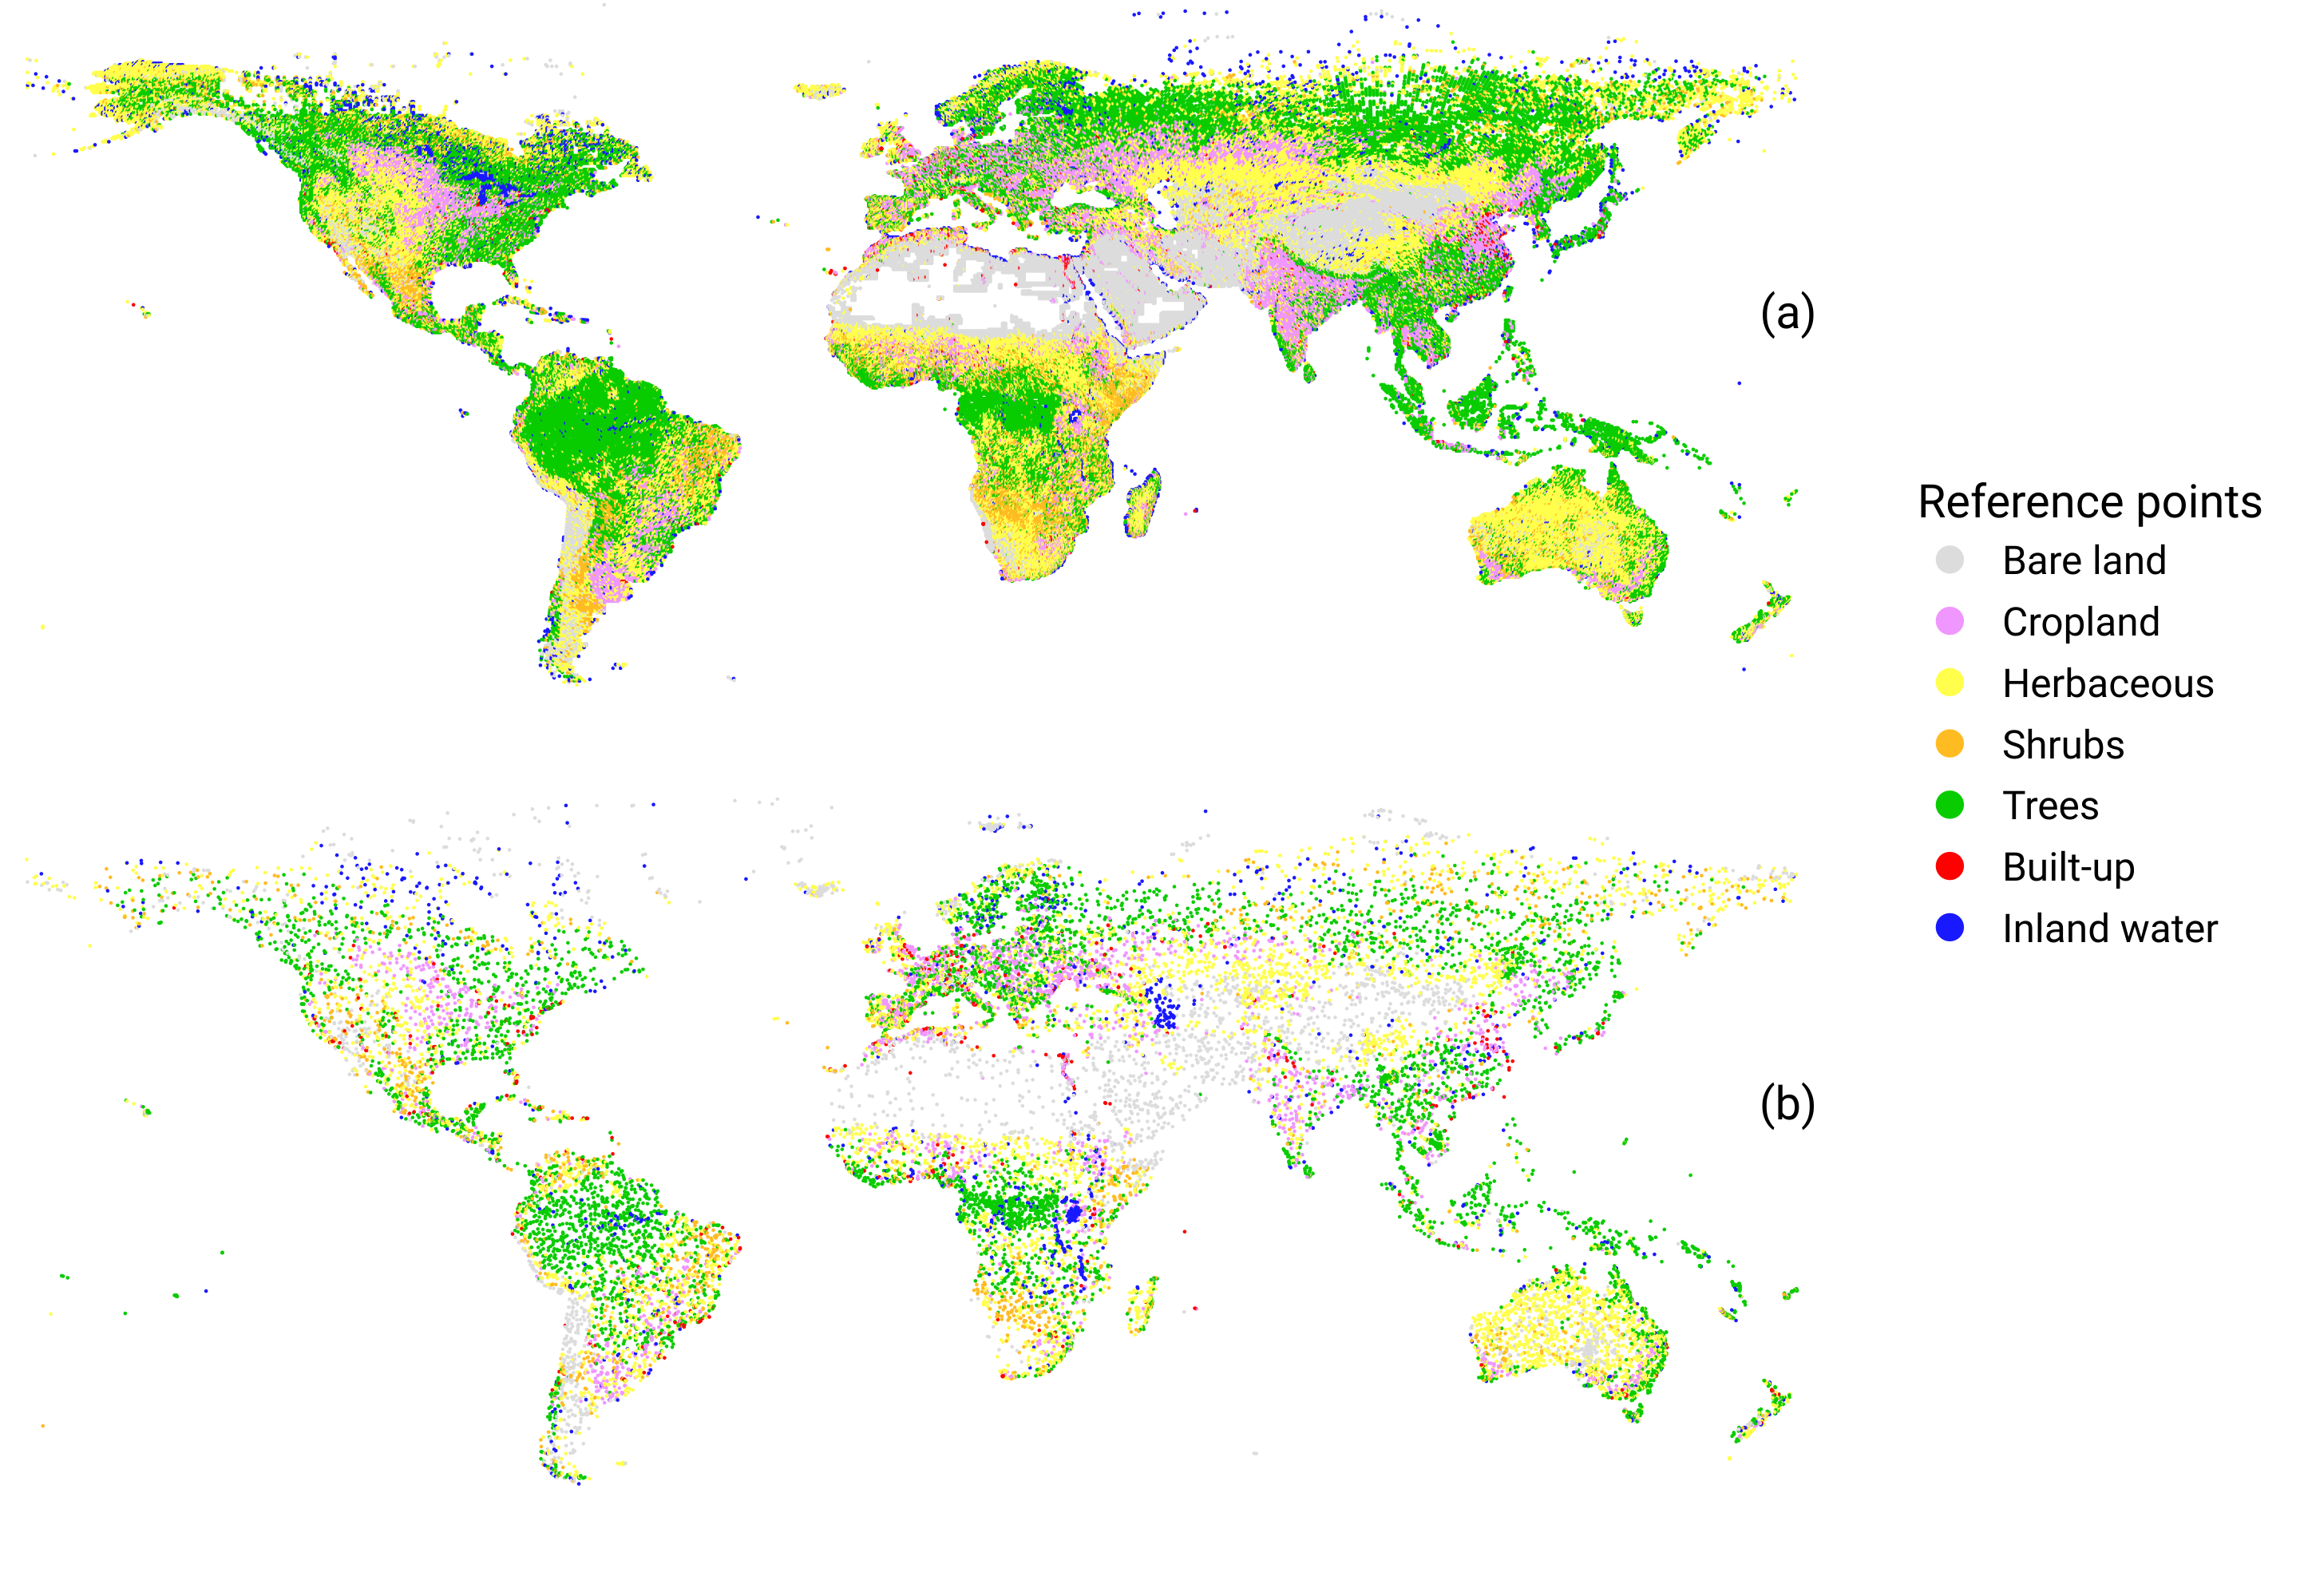
\includegraphics[width=\textwidth]{article-figures/maps/2020-10-12-training-and-validation}
 \caption{Sample points representing 100x100~m areas at which land cover reference data was used in the study. The colours represent the dominant land cover class at each point. (a): training dataset, collected by \gls{IIASA}, 138\,164 points used in this study. (b): validation dataset, collected by \gls{WUR}, 20\,705 points used in this study. Both datasets were collected as part of the \ac{CGLS-LC100} project \citep{buchhorn_copernicus_2020}.}
 \label{fig-reference-data}
\end{figure}

\subsection{Model training features}

See figure \ref{fig-processing} for an overview of the whole processing chain used in this study.
The processing was carried out in R \citep{r_2019} and the resulting code has been made openly available in \citet{dainius_masiliunas_2020_3973123}.

To train the models and predict land cover fractions in unsampled locations, six groups of features were used: vegetation indices, temporal metrics, terrain metrics, soil metrics, climate metrics and location data (see supplementary material, table S1).
These features had to be preprocessed before they could be input into the models.

\begin{figure}
 \centering
 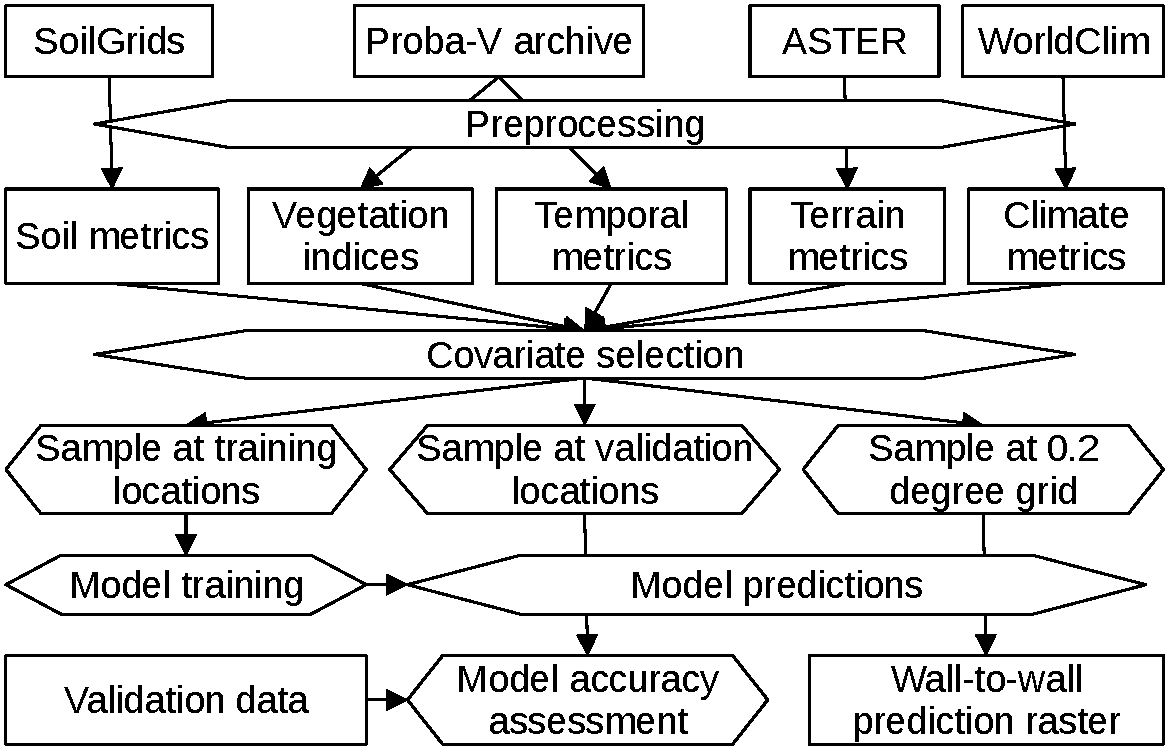
\includegraphics[width=0.6\textwidth]{article-figures/flowcharts/2020-07-10-flowchart}
 \caption{Processing workflow, from the raw input data to model accuracy assessment and wall-to-wall map output.}
 \label{fig-processing}
\end{figure}

% \begin{table}
% \centering
%     \begin{tabular}{llp{6cm}}
%          \toprule
%          \textbf{Category} & \textbf{Number} & \textbf{Data source} \\
%          \midrule
%          Spectral & 22 & PROBA-V 100m \ac{TOC} reflectance v1.02 \citep{probavguide2} \\
%          Harmonic & 9 & PROBA-V 100m \ac{TOC} reflectance v1.02 \citep{probavguide2} \\
%          Terrain & 4 & ASTER GDEM V003 \citep{ASTGTM003} \\
%          Climate & 21 & WorldClim 2.0 \citep{worldclim2} \\
%          Soil & 8 & SoilGrids \citep{hengl_soilgrids250m_2017} \\
%          Location & 3 & None (intrinsic) \\
%          \bottomrule
%     \end{tabular}
%     \label{tab-inputdata}
%     \caption{Data sources for the features input into the model.}
% \end{table}

\label{sec-temporal-filter}

We chose to use the entire archive (2014-03-11 to 2019-07-16) of the PROBA-V 100~m Level~3 Top-of-Canopy 5-day composite product \citep{dierckx2014probav,probavguide2} for this study.
The PROBA-V archive provides a relatively long history of frequent (daily or 2-day) observations, which is beneficial for time series analysis, as there are more observations of the land surface in cloudy areas, and a dense time series of observations can be acquired to generate robust temporal metrics.
While the reference data corresponded to the land cover at the year 2015 specifically, we chose to use the whole time series of PROBA-V data to obtain more robust statistics for the temporal metrics.
The long time series makes the temporal outlier filtering step more reliable, increases the robustness of the fitted harmonic model, and removes the effects of interannual variability and seasonality in the calculated descriptive statistics, as described in the following sections.
Land cover change is a relatively rare phenomenon, according to tests performed in the making of \gls{CGLS-LC100} collection 3, and so we expected that the difference caused by land cover change to the input data would be smaller than the margin of error of the model output.
Nevertheless, this may result in poorer model performance compared to if up-to-date reference data for each year would be available.

We masked out the clouds from the time series of each of the four PROBA-V spectral bands, first by applying the status mask provided with the product itself, and then by running a temporal cloud filter to remove the remaining outliers that were further than 2 standard deviations away from the \ac{LOESS} curve fitted over the blue reflectance band.
We then used the resulting cloud-free time series to generate the following \glspl{VI}: \gls{NDVI}, \gls{NDMI}, \gls{EVI}, \gls{OSAVI} and \gls{NIRv}.
These \glspl{VI} are commonly used in land cover mapping to aid in discerning the vegetation classes among each other.
Next, we used the \gls{VI} time series to calculate the descriptive statistics (median and interquartile range) over the whole time series, as well as for each phenological season separately.
We included the resulting metrics as vegetation index features.
Next, we ran harmonic analysis \citep{jakubauskas2001harmonic} on NDVI in order to decompose the time series into sine and cosine components for two frequency orders (annual and semiannual), as well as the trend and intercept of the model.
The temporal metrics from the harmonic model quantify the seasonality of the area and allow differentiating between vegetation with different seasonality, such as crops.
From this harmonic analysis we obtained the minimum and maximum values of the \gls{NDVI} time series, which we included as additional vegetation index features.
We also obtained the the trend and intercept components from the harmonic model.
Lastly, we calculated the phase and amplitude for the two harmonic orders from the respective sine and cosine components of the model.
We used these sine, cosine, trend and intercept components, as well as the phase and amplitude of the two harmonic orders, as temporal features in our study.
For a list of features that were ultimately used as input to the models, see supplementary material, table S1.

To generate elevation features, we obtained the ASTER GDEM v003 \citep{ASTGTM003} product (30 m) and resampled it to the PROBA-V 100~m grid.
We used the result directly as the terrain elevation feature.
In addition, we used \gls{GDAL} \citep{gdal} to calculate terrain parameters out of elevation: slope, aspect and \ac{TPI}.

We chose the WorldClim~2.0 30~second product \citep{worldclim2} as a source of climate features.
It includes monthly temperature, precipitation, solar radiation, wind speed and water vapour pressure data.
In addition to these features, we calculated 19 bioclimatic parameters from the data, using the \cran{dismo} package \citep{dismo}.
We also calculated some additional biophysical parameters, namely all of the climate variables during the coldest, warmest, driest and wettest months of the year at each location, as well as the yearly averages of the climate variables.

We used SoilGrids \citep{hengl_soilgrids250m_2017} to obtain features related to soils.
SoilGrids is based on a random forest model that predicts soil properties at various soil depths globally at a 250~m resolution.
In the creation of SoilGrids, a land cover map (based on MODIS) had been used, and so, in order to avoid circular inference, the features that are significantly influenced by the land cover map as detailed in \citet{hengl_soilgrids250m_2017} were excluded.
The soil taxonomy features were also excluded, since they are categorical derivatives from the numerical soil property data and thus do not contribute to land cover fraction prediction.

Lastly, we also included the latitude, longitude and absolute latitude of the reference points as location features when training the models, so that the models could learn spatial patterns.

\subsection{Feature selection}
\label{sec-covariate-selection}

In total, we generated 313 features in preprocessing.
However, many of them were collinear with one another.
Multicollinearity prolongs training time for machine learning models and leads to unreliable coefficient estimation and increased error variance for linear models.
Thus, we employed variable selection to remove collinear features before predicting the land cover fractions.
Features that had a Pearson's correlation coefficient $r$ \citep{pearson_notes_1895} above 0.9 were excluded in an iterative process.
After that, features with a Spearman's rank correlation $\rho$ \citep{spearman1904rank} above 0.9 were likewise excluded.

We manually selected the features to exclude, to avoid interpretation difficulties that arise from automatic selection procedures.
The majority of the collinear features were soil metrics predicted at different depths.
Therefore, we left in the 10 cm depth features, and excluded the other depths, as long as $r$ was above 0.9.
Similarly, climate data was collinear between subsequent months. Thus January and July data was preferred, as these months represent different extremes of the year and are less correlated with data of the other months.
Our initial correlation analysis also showed that the spectral bands of PROBA-V were highly correlated with each other as well as to \glspl{VI}, so we only used \glspl{VI} as features.

After the feature selection process, 67 features remained.
These features include data from each of the feature categories.
See supplementary material, table S1 for an overview of all of the features that remained and thus used in model training and prediction.

\subsection{Land cover fraction mapping methods}

We compared a wide array of machine learning regression methods for deriving land cover fractions.
The tested methods can be broadly divided into three types: linear models, machine learning models based on \glspl{CART}, and machine learning models not based on \glspl{CART}.
See table \ref{tab-methods} for the full list of methods that we compared in this study.
In addition, as a baseline we also compared the results with a trivial equal proportion model (all fractions always predicted to be equal, namely $\frac{100\%}{7}\approx14.29\%$).
We tuned each algorithm to select optimal parameters, and postprocessed the output of each algorithm as necessary to ensure that all land cover fractions in each pixel add up to 100\%.
Namely, if the model output for any class was outside of the 0-100\% range, the values were clamped to that range, and if the values did not add up to 100\%, they were linearly rescaled so that they would.
All of the model building and data analysis was performed using the free and open-source statistical software R \citep{r_2019}.

\begin{table}
\centering
    \begin{tabular}{m{4cm}ll}
         \toprule
         \textbf{Category} & \textbf{Name} & \textbf{Reference} \tabularnewline
         \midrule
         Linear models &
         \begin{tabular}{@{}l@{}}
         \Glsentryfull{FNC}\tabularnewline
         \Glsentryfull{GLM}\tabularnewline
         \Glsentryfull{PLS} regression \tabularnewline
         Lasso regression \tabularnewline
         \Glsentryfull{MLR}
         \end{tabular}
         & 
         \begin{tabular}{@{}l@{}}
         \citealt{keller_fuzzy_1985} \tabularnewline
         \citealt{neter_applied_1996} \tabularnewline
         \citealt{wold_pls-regression_2001} \tabularnewline
         \citealt{tibshirani_regression_1996} \tabularnewline
         \citealt{theil_multinomial_1969}
         \end{tabular}
         \tabularnewline \midrule
         Machine learning models based on decision trees &
         \begin{tabular}{@{}l@{}}
         \Glsentryfull{RF} regression\tabularnewline
         Cubist regression
         \end{tabular}
         &
         \begin{tabular}{@{}l@{}}
         \citealt{breiman2001random} \tabularnewline
         \citealt{cubist}
         \end{tabular}
         \tabularnewline \midrule
         Other machine learning models &
         \begin{tabular}{@{}l@{}}
         \Gls{MLP} \glsentryfullpl{NN}\tabularnewline
         \Glsentryfull{SVM} regression
         \end{tabular}
         & 
         \begin{tabular}{@{}l@{}}
         \citealt{dreyfus_artificial_1990} \tabularnewline
         \citealt{suykens_least_1999}
         \end{tabular}
         \tabularnewline \midrule
         Ensemble learning &
         Super Learner
         & 
         \citealt{laan_super_2007}
         \tabularnewline \bottomrule
    \end{tabular}
    \caption{List of regression methods for land cover fraction estimation tested in this study.}
    \label{tab-methods}
\end{table}

\subsubsection{Linear models}

We chose to compare five types of linear models, to have a baseline for a comparison with the nonlinear machine learning models.
The most simple model we selected was the \gls{GLM} \citep{neter_applied_1996}, also known as multivariate linear regression.
It is an extension to the standard linear regression that allows for multiple outcomes, and is implemented in base R \citep{r_2019}.
Next, we tested two linear models that include input data regularisation in the model itself: lasso regression \citep{tibshirani_regression_1996}, implemented in the \cran{glmnet} package \citep{glmnet}, and \gls{PLS} regression \citep{wold_pls-regression_2001}, implemented in the \cran{pls} package \citep{pls}.
We also tested \gls{MLR} \citep{theil_multinomial_1969}, provided by the \cran{nnet} package \citep{nnet}.
\gls{MLR} is usually used for classification and is fit using land cover class labels rather than fractions, but the output includes probabilities for each class that add up to 100\%.
We fit \gls{MLR} using the dominant land cover class as a label for the pixel and used the class probabilities as a proxy for land cover fractions.
Lastly, we tested \gls{FNC} regression \citep{keller_fuzzy_1985}, also called fuzzy nearest prototype, fuzzy $c$-means or fuzzy $k$-means, which is provided in the \cran{GSIF} package \citep{hengl2004fuzzycmeans}.
It is a simple regression method, where the land cover fractions in a pixel are determined by the distance of the pixel from the centroids of each class in feature space.

%The \gls{GLM} \citep{neter_applied_1996}, also known as multivariate linear regression, is an extension to the standard linear regression that allows for multiple outcomes.
%In this study, we used a \gls{GLM} as a baseline model.
%We also tested whether dropping any additional features from the model would result in better predictions, using a sphericity test with Greenhouse-Geisser correction \citep{greenhouse_methods_1959} to compare models with different features.
%However, only three features could be dropped and it did not improve the predictions, therefore we decided to keep all the features in the model.
%\Gls{GLM} is implemented in base R \citep{r_2019}.

%Ridge regression is a linear model regularisation method which reduces large coefficients of model features in order to prevent overfitting.
%Lasso regression is based on the same principle, except it reduces the coefficients of each model feature to zero if the absolute sum of coefficients is above a threshold, thus acting as a variable selection method.
%Elastic net regression is a method combining the two, where model coefficients may be reduced or set to zero.
%This has the effect of the coefficients of correlated features being set to a similar value.
%We chose lasso regression \citep{tibshirani_regression_1996}, so that it would be possible to identify if there are any features that could be further omitted in addition to ones dropped in section \ref{sec-covariate-selection}.
%The $\lambda$ parameter was chosen using cross-validation.
%The lasso regression was performed using the \cran{glmnet} package \citep{glmnet}.

%\Gls{PLS} regression \citep{wold_pls-regression_2001} is a concept related to principal component regression and also aims at reducing the input features into latent variables that explain the most variance of the response variable in multidimensional space.
%As such, it is well suited for multicollinear data.
%\ac{PLS} regression was performed using the package \cran{pls} \citep{pls}.

%All of the aforementioned linear models do not normalise the output to add up to 100\%, and also allow negative predictions.
%Therefore for these models, all predictions < 0 were set to 0, and then all values were linearly rescaled per each prediction to add up to 100\%.

%\Gls{FNC} regression \citep{keller_fuzzy_1985}, also called fuzzy nearest prototype, fuzzy $c$-means or fuzzy $k$-means, is a simple regression method where the pixel's membership of a class is determined by the distance of the pixel from each class centroid in feature space.
%This method always produces output that sums to 100\%.
%In this study, we used an implementation adapted from the package \cran{GSIF} \citep{hengl2004fuzzycmeans}.
%We tested both using a logistic regression to estimate the class centroids, as well as using a weighted average of the training data to do so, and ended up using the latter method as the result was more accurate.

%Lastly, we tested \gls{MLR} \citep{theil_multinomial_1969}.
%While logistic regressions are most commonly used for classification tasks, the output of a multinomial regression itself is the probability of a pixel to belong to each of the defined classes.
%This probability can be used as a proxy for the fraction of the pixel that the class covers.
%These probabilities always add up to 100\%.
%However, an \gls{MLR} can only be trained on labelled data, rather than fractions.
%Therefore the target (label) input for the \ac{MLR} was the name of the dominant land cover fraction of each pixel.
%This does not guarantee that the pixels that the model was trained on were pure endmembers, but it allows the model to learn from a much larger dataset compared to using just the pure pixels.
%The logistic regression implementation was provided by the \cran{nnet} package \citep{nnet}.

\subsubsection{Non-tree machine learning methods}

\Glsentryfullpl{NN} are a promising technique for land cover fraction mapping, as they allow both multiple inputs and multiple outputs, and, using the softmax activation function, also ensures that the result sums up to 100\% with no need for additional postprocessing.
In this study, after performing tuning, we ended up using a \glsentryfull{MLP} \citep{dreyfus_artificial_1990} with three hidden layers with 128, 64 and 32 neurons per layer respectively.
We used the Nadam optimiser \citep{dozat_incorporating_2016} with \gls{MAE} as the loss function to optimise the \gls{NN}, and softmax activation for the output.
The models were trained using the \cran{keras} package \citep{keras}, built upon TensorFlow that enables the use of a graphics processing unit to accelerate the \gls{NN} training process.

\Glsentryfullpl{SVM} are machine learning models that attempt to find the optimal boundary between the class clusters in feature space by constructing a dividing hyperplane.
For land cover fraction classification, we used \gls{SVM} regression based on Least Squares \gls{SVM} \citep{suykens_least_1999}.
As \gls{SVM} models are univariate, we used the binary relevance method \citep{karalas2016br}: training separate models per class that predict a single class, and then combining the results.
We found the package \cran{liquidSVM} \citep{liquidSVM} suitable for this purpose, as it is optimised for processing large datasets such as ours.

\subsubsection{Tree-based machine learning methods}

\Glsentryfull{RF} regression is a popular method for land cover classification that works by building a number of \gls{CART} decision trees based on random subsets of the input training data, and taking the mean or median of the ``votes'' of these individual decision trees \citep{breiman2001random}.
\ac{RF} is univariate, therefore we again used the binary relevance approach.
The processing was done using the \cran{ranger} package \citep{ranger}.

Lastly, we tested Cubist regression \citep{cubist}.
It is based on \gls{RF} regression, but instead of using a threshold of a feature to split the decision tree, Cubist uses a linear regression based on a subset of the data relevant for the split in question.
In addition, it features committees, a boosting technique that iteratively trains trees so as to learn from the previously generated ones.
Model tuning led to us using 10 committees.
Cubist predictions were also made using the binary relevance method.
The algorithm is provided by the \cran{Cubist} package \citep{cubistpackage}.

\subsubsection{Ensemble learning}

Lastly, we made an ensemble from the two machine learning models that produced the lowest \gls{RMSE} and \gls{MAE} respectively.
We used the \cran{sl3} package \citep{sl3} to create a hierarchical ensemble, where the two models were cross-validated using 10-fold cross-validation to obtain relative weights of each model for each land cover class, following the super learner algorithm \citep{laan_super_2007}.
The predictions of the two models, along with the weights of the models, were then used as input features for another \gls{RF} regression metalearner.
The output from this metalearner is the final prediction of the whole ensemble.
As the ensembled methods are univariate, we used the binary relevance method in this case as well.

%\subsubsection{Other methods}

%Additional methods were considered, but in the end turned out to be unworkable with our dataset.
%Multivariate \gls{RF} is available in R provided by the \cran{MutivariateRandomForest} package \citep{MultivariateRandomForest}, which would potentially allow better results than using regular \gls{RF} with binary relevance.
%However, it is not optimised for large datasets, which did not allow to train it on more than 2000 samples at a time, making it incomparable to the rest of the tested methods.

%Another model that was considered was \cran{SuperLearner} \citep{SuperLearner}, an ensembling method that can combine multiple of the tested methods into one model, giving models different weights according to how well they are known to perform for a given task.
%Here we ran into similar issues, as cross-validation is required for each model to train, which increases processing time dramatically.
%Attempts to reduce training time by lowering the number of folds resulted in worse results than when using a single classifier.

%Lastly, multiple-endmember spectral unmixing using non-negative least squares \citep{franc2005sequential} was also attempted, but the results were significantly worse than even the equal proportions model, possibly because the class fractions are not a linear combination of the features.

\subsection{Multi-step approach to account for value imbalance}
\label{sec-multistep}

After determining the method with the lowest \gls{RMSE}, we attempted to improve it further in an attempt to solve the dataset balance issue, namely the high frequency of 0\% and 100\% fractions.
As the dataset describes fractions of each land cover class at each point, most of the locations consist of a mix of only a few classes, and the fraction of the rest of the classes is zero at that location.
If the pixel is pure, then one land cover class will be 100\% and the rest 0\%, which is also a common case.
This leads to the dataset getting dominated by zeroes.
In that case, minimising the objective function of a machine learning model leads to prioritising predicting 0\% fractions well, and ignoring the prediction errors in the middle of the 0-100\% range.
This is not desirable for users of land cover fraction data, as the added value of fraction information is the information about the middle of the range; otherwise, discrete classification would be just as good.
Conversely, 0\% by itself is rarely predicted precisely, because when the value is uncertain, predictions tend towards the mean.
Therefore we tried several approaches to deal with data imbalance by employing a hierarchical combination of machine learning models.

Taking the algorithm with the lowest \gls{RMSE}, we compared three approaches.
(a): a single regression model trained on all data.
(b): a two-model approach in two steps.
Step 1: a binary classification model for each class to predict zeroes, trained on a generated dataset that, based on the land cover fraction values, had labels ``zero'' and ``non-zero''.
Step 2: a model to predict non-zeroes, trained on all of the non-zero fraction values.
For the combined prediction, all points that were predicted as ``zero'' in step 1 were set to 0\%, otherwise the value from the model in step 2 was used.
(c): a three-model approach using three steps.
Step 1: a binary classification model to predict pixel purity (i.e. whether we face a classification or a regression problem), trained on a generated dataset that had labels ``pure'' for points that had a single land cover fraction above a purity threshold, e.g. 95\%, and ``non-pure'' for points that do not.
Step 2: a model to perform regression on mixed pixels (as determined in step 1).
Step 3: a model to perform classification on pure pixels (as determined in step 1), resulting in a prediction of 100\% fraction of the predicted discrete class and 0\% fractions for all other classes.
The combined prediction is the combination of the results of steps 2 and 3, as determined by step 1.

For the three-step approach, we also tested the effect of the fraction threshold for when we consider a pixel ``pure''.
The lower the threshold, the more pixels are considered pure and the more often the classification model will be selected, as opposed to the regression model.
We also evaluated the accuracy metrics of the separate steps of the multi-step models.

Lastly, we compared the results of our proposed multi-step approach with an approach that uses the median for ensembling tree votes, instead of the mean.
The median vote leads to predicting the extreme fractions of 0\% and 100\% more often, since if the majority of the decision trees vote for one of the two extremes, it gets selected as the output value.
Finally, we also investigated the combination of both approaches.

\subsection{Accuracy assessment}

To assess the performance of the models, we used a number of statistical measures.
We started with the statistics of assessing land cover fraction model accuracy that are the most commonly used in this field: \glsentryfull{RMSE}, \glsentryfull{MAE} and \glsentryfull{ME}.
\gls{MAE} represents the average difference between the predicted and the reference land cover fractions.
In our case, its unit is percentage points.
\gls{RMSE} squares the errors, therefore giving a larger penalty for large errors, and thus is always higher than \gls{MAE}.
These statistics are relatively straightforward to calculate and interpret.
In the case of land cover fraction mapping, \gls{RMSE} is very sensitive to errors where a pixel is entirely mapped as a different class (i.e. 100\% instead of 0\%).
\gls{MAE} is more lenient and not as influenced by a small number of such large misclassifications.
Thus it is more indicative of the overall model accuracy, whereas \gls{RMSE} is more indicative of the presence of large errors.

We calculated \gls{RMSE}, \ac{MAE} and \ac{ME}, both separately per class, and also pooled overall.
These overall measures were calculated by taking the mean of all class points pooled together, rather than taking a mean of the per-class means.
In addition, we calculated the \gls{RRMSE}, \gls{RMAE} and \gls{RME} for each class by dividing the absolute measures by the mean fraction of each class.
The relative statistics give an extra penalty for poor predictions of rare land cover fractions (i.e. those that are absent from most pixels), to account for the issue that a prediction of constant 0\% would lead to low \gls{RMSE} and \gls{MAE} for rare class fractions.

Next, we estimated the goodness of fit of the models by calculating the coefficient of determination $R^2$ of the models in two ways.
The first way is \gls{NSE} \citep{nash1970river}, which is equivalent to an $R^2$ of a linear regression model whose intercept and slope terms are predetermined and are equal to 0 and 1, respectively.
This metric shows how far away the predicted values are from the 1:1 line with the reference values.
The value range of \gls{NSE} is $(-\infty, 1]$, where a value of 0 means that the predicted values are no better than predicting the mean value.
The second way is to calculate the $R^2$ of an Ordinary Least Squares regression that estimates the intercept and slope, rather than presetting it.
This method always gives higher $R^2$ values than \gls{NSE}, as it allows the regression line to have more flexibility.
The two ways of estimating the coefficient of determination are herewith represented as $R^2_{NSE}$ and $R^2_{OLS}$, respectively.

Furthermore, we calculated a \gls{SCM} \citep{silvan-cardenas_sub-pixel_2008}, and the metrics derived from it: \ac{OA}, as well as \ac{PA} and \ac{UA} per class.
The \gls{SCM} is an adaptation of the confusion matrix concept to fractional data.
We used the MIN-PROD composite operator as recommended by \citet{silvan-cardenas_sub-pixel_2008}.
When using this operator, the diagonal of the matrix expresses the maximum overlap (agreement) of the target and predicted class fractions, and the off-diagonal is an expression of which classes the non-overlapping fractions should belong to by calculating the expected value of overlap (product of reference and predicted class fraction).
For instance, a pixel of 60\% grass and 40\% shrub, when predicted as 40\% grass and 60\% shrub, would have $min(60\%, 40\%)=40\%$ in the diagonals and $\frac{20\%\times20\%}{20\%}=20\%$ in the off-diagonals.
For cases where the allocation of the overestimated and underestimated parts of the fraction do not have a unique solution, the \ac{SCM} indicates the expected value and an associated uncertainty measure.

Moreover, to show the variation in predicted land cover fraction values depending on the magnitude of the fractions, we produced boxplots showing the distribution of the predictions.
The boxplots are binned for each 10\% of the predictions.
The 1:1 line indicates how well do the distributions of the predictions and the reference data match.

Lastly, we produced spatial residuals, i.e. the overestimation and underestimation of each class fraction for each validation point.
We rasterised the result into a map for ease of view.
If multiple points fell into the same raster cell, we reported the mean value.

To put our results in a wider context, we compared them with the currently available global products for specific land cover classes.
For this comparison, we used the same validation dataset as for our models.
Since the validation dataset reflects land cover of the year 2015, we chose to compare our results with four products produced for or around the year 2015.
Therefore we chose the \gls{GFCC} forest cover product for 2015 \citep{townshend_global_2017}, the \gls{GSW} water occurrence history product for 2015 \citep{pekel_high-resolution_2016}, and two products for the comparison with the built-up class: \gls{GHSL} built-up for 2014 \citep{corbane_automated_2019} and \gls{FROM-GLC} impervious surface change layer for 2015 \citep{gong_annual_2020}.
As the latter two products show the change in built-up cover over time, we reclassified them to have a value of 100 if the area was built-up in 2014 or 2015, respectively.
For \gls{FROM-GLC}, we assumed that areas that had been covered by impervious surface at any time prior to 2015 continued to be covered by impervious surface in 2015.
\gls{GSW} data was also reclassified to 100 if the water was permanently present and 50 if it was seasonally present.
Next, for validation purposes we resampled each product to the PROBA-V 100 m grid using the bilinear resampling method, so that the cover fractions get aggregated over the same areas as our own data.
Then we compared the product values with our validation data point values.

\subsection{Feature importance}

To calculate feature importance, we performed permutation importance on the model that had the lowest \gls{MAE}.
We shuffled the values of each feature in turn, and the models made predictions based on all of the features, including the shuffled one.
This results in a decrease in the accuracy of predictions, as the feature in question no longer contains meaningful information.
We then recorded the resulting increase in \gls{MAE} compared to the validation set as a measure of feature importance, both per class and overall for all classes combined.

\section{Results}

\subsection{Method accuracy comparison}

The overall accuracy statistics of the compared models are reported in table \ref{tab-accuracy}, and per-class statistics in figure \ref{fig-models}.
Overall, \gls{RF} regression achieved the highest accuracy: by \gls{RMSE} when using a single model and a mean vote, and by \gls{MAE} when using a median vote.
The combination of the three-step model and the median vote resulted in a decrease in \gls{RMSE} without impacting \gls{MAE}.

The results show that the $R^2$ statistics, especially $R^2_{NSE}$, are in agreement with the \gls{RMSE} statistics, and the \glsentryfull{OA} from the \glsentryfull{SCM} is in agreement with the \gls{MAE} statistics.
$R^2$ is a representation of how closely the predictions correlate with the validation data, therefore big outliers have a large effect on the value.
The \gls{SCM} does not take this into account, as it does a comparison on the overlap of fractions in each pixel, which doesn't apply an extra penalty for large errors.

The baseline models that performed the best were the two tree-based machine learning models: \gls{RF} regression and Cubist.
Both of these models are univariate, therefore predictions per class had to be made using the binary relevance method (one model per class).
This shows that despite the limitations of the binary relevance method, namely that each model is only trained on the fractions of its own class and has no knowledge of the fractions of the other classes, and the need for a rescale step to make sure the fractions sum up to 100\%, the advantages of these machine learning models and the flexibility of fitting the models for each class outweigh the disadvantages of the binary relevance method.

The super learner method that combines both \gls{RF} regression and Cubist regression resulted in a model that is in between the two ensembled models in terms of accuracy.
Its \gls{RMSE} was below that of Cubist regression, but above that of \gls{RF} regression.
Conversely, the \gls{MAE} was below that of \gls{RF} regression (single model), but above that of Cubist regression.
This shows that the metalearner (another \gls{RF} model) could not differentiate between the two ensembled models well enough to select the model that is the most accurate for a given class.
Rather, it weighted in both of the models' predictions, losing the advantages of the models when taken separately.

The linear statistical models (\gls{GLM}, \gls{PLS}, Lasso regression and \gls{MLR}) performed the worst, as they are limited to a linear approach.
The results of all of the linear models were very similar.
There was no added value to \gls{PLS} and Lasso regressions over the basic \gls{GLM}.
This is likely due to the additional preprocessing step of feature selection, as detailed in section \ref{sec-covariate-selection}.
Lasso and \gls{PLS} regressions are extensions to \gls{GLM} that include a regularisation step, which proved to be unnecessary if all of the highly correlated features are already manually removed.

\Gls{FNC} was the model that performed the worst out of the non-trivial models tested.
This indicates that the shape of the feature data in feature space is too complex to capture merely with a centroid approach.
This is further evidenced by a much better result obtained by the binary relevance \gls{SVM} model, which works on a similar principle but can capture more complex shapes.

\Gls{MLP} \glspl{NN}, despite being a multivariate machine learning model, performed worse than all of the tested binary relevance methods.
Nevertheless, it performed better than all of the multivariate linear models.

\begin{table}
\centering
%\adjustbox{max width=0.5\textwidth}{
\begin{tabular}{lllllll}
\toprule
\textbf{Model} & \textbf{\ac{RMSE} (\%)} & \textbf{\ac{MAE} (\%)} & $\mathbf{R^2_{NSE}}$ & $\mathbf{R^2_{OLS}}$ & \textbf{\ac{OA} (\%)} & \textbf{Kappa} \\
\midrule
Equal proportions
& 29.9  & 21.4  & 0     & — & 26±5  & 0.13±0.07 \\
\Gls{FNC}
& 24.4  & 13.5  & 0.33  & 0.35 & 53±4  & 0.42±0.06 \\
\Gls{GLM}, \Gls{PLS}, Lasso
& 21.6  & 12.7  & 0.48  & 0.49 & 56±4  & 0.43±0.05 \\
\Gls{MLR}
& 21.6  & 12.1  & 0.48  & 0.48 & 58±4  & 0.46±0.06 \\
\Gls{MLP} \glspl{NN}
& 22.7  & 9.2   & 0.43  & 0.52 & 68±1  & 0.57±0.02 \\
\Gls{SVM} regression
& 20.7  & 8.9   & 0.52  & 0.56 & 69±2  & 0.58±0.03 \\
Cubist regression
& 18.1  & 8.1   & 0.63  & 0.65 & \textbf{72±2}  & 0.63±0.03 \\
\Gls{RF} regression
& \textbf{17.3}  & 9.4   & \textbf{0.66}  & \textbf{0.67} & 67±4  & 0.57±0.05 \\
\ensuremath{''}
only RS features
& 18.4  & 10.3  & 0.62  & 0.64 & 64±4  & 0.54±0.05 \\
\ensuremath{''} two-step
& 19.9  & 8.2   & 0.56  & 0.60 & 71±2  & 0.62±0.02 \\
\ensuremath{''} three-step
& 19.4  & 8.4   & 0.58  & 0.60 & 71±3  & 0.62±0.04 \\
\ensuremath{''} median vote
& 20.7  & \textbf{7.9}   & 0.52  & 0.60 & 71±1  & 0.63±0.02 \\
\ensuremath{''} \ensuremath{''} two-step
& 20.0  & 8.1   & 0.54  & 0.60 & \textbf{72±1}  & 0.63±0.02 \\
\ensuremath{''} \ensuremath{''} three-step
& 20.2  & \textbf{7.9}   & 0.54  & 0.60 & \textbf{72±2}  & \textbf{0.64±0.02} \\
Cubist + RF ensemble
& 17.7  & 8.6   & 0.65  & 0.65 & 70±3 & 0.61±0.04 \\
\bottomrule
\end{tabular}
%}
\caption{Accuracy statistics of the tested models. Best performing statistics are highlighted. ``Only RS features'' stands for a model trained only with \glspl{VI} and temporal metrics.}
\label{tab-accuracy}
\end{table}

\begin{figure}
    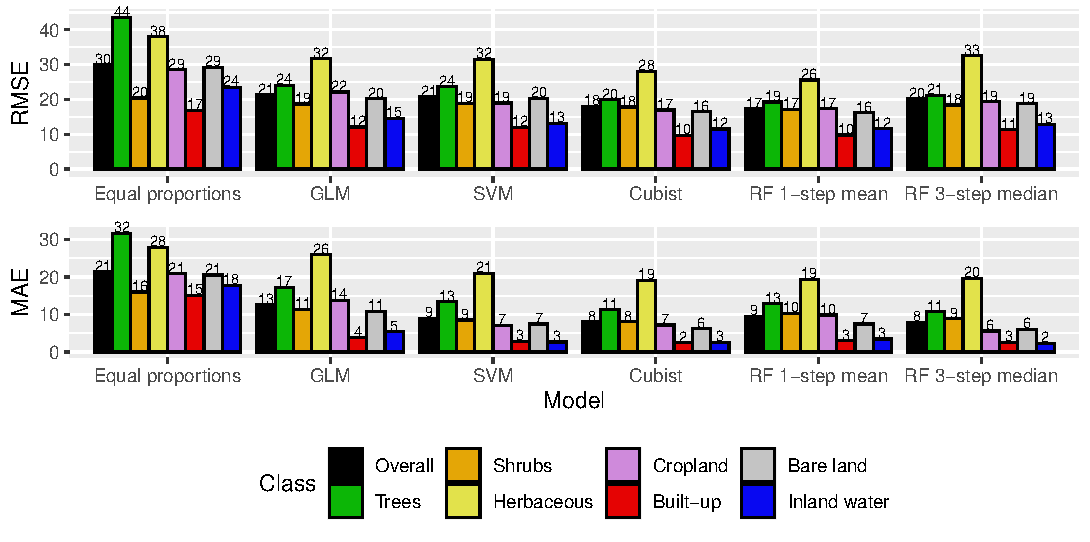
\includegraphics[width=\textwidth]{article-figures/barplots/2020-06-03-model-comparison-bar}
    \caption{Comparison of absolute \gls{RMSE} (top) and absolute \gls{MAE} (bottom) per class of the best performing models in their category, and the equal proportions solution as a reference.}
    \label{fig-models}
\end{figure}

%There was a trade-off between optimisation for \gls{MAE} and \gls{RMSE}, i.e. between penalising for large errors or not.
%Models that had lower \gls{MAE} were more crisp, whereas models with lower \gls{RMSE} were more fuzzy.
%Models that achieved lowest \gls{MAE}, in cases of high uncertainty tended to predict 100\% fractions more often, but risk predicting 100\% of the wrong class, whereas models with lowest \gls{RMSE} would predict a mix of all classes that could be within the pixel, thus more often making predictions that are partially but not completely incorrect.
%Therefore models optimised for \gls{RMSE} are closer to a probabilistic view of land cover, whereas models optimised for \gls{MAE} are more representative of the best guess of the model for the most likely pure class of the pixel.

All tested models had lower accuracy when estimating the cover fractions of vegetation classes (herbaceous, trees, crops, shrubs), compared to the non-vegetated land cover (inland water, built-up, bare land), as shown in figure \ref{fig-models}.
This was exacerbated by the imbalance in class distribution: the built-up class is rare and very rarely forms a majority, therefore a prediction of 0\% leads to a perfect prediction most of the times, and even if it does not, the error is low.
In contrast, tree cover had a lot more balanced distribution of fractions, including a large number of pure pixels, which leaves no such trivial solution.
The \gls{RRMSE} and \gls{RMAE} statistics show this (see supplementary material, figure S1): the tree cover prediction has low relative error given its high mean value (32\%), whereas the built-up class is the most challenging to predict according to \gls{RRMSE} given its low mean value (3\%).
The shrub cover fraction is also very challenging to predict, since it had the highest \gls{RMAE} and none of the models showed large improvements in \gls{RMSE} compared to the equal proportions model.
There were only moderate improvements for predicting the herbaceous vegetation fraction as well.
In contrast, most models were a significant improvement in predicting tree, built-up, water and bare cover fractions compared to the equal proportion model, indicating that the features used to train the models were useful to distinguish these classes from the others and to quantify their proportions in each pixel.

\subsection{Zero inflation adjustment with multi-step models and median voting}

We investigated two ways to adjust for the issue of zero inflation in the training data.
First, we used a median vote instead of a mean vote for ensembling decision tree votes in \gls{RF} regression, so as to predict exactly 0\% and 100\% more often.
Second, we used our proposed multi-step model approach as detailed in section \ref{sec-multistep}.
The overall results can be seen at the bottom of table \ref{tab-accuracy}, whereas per-class results can be seen in figure \ref{fig-randomforest} and supplementary material, figure S2.

The median voting approach resulted in significantly more predictions of 0\% and 100\% class fractions, therefore the output looked closer to a discrete classification map compared to mean voting.
Since these two most common values were predicted precisely much more often, \gls{MAE} reduced.
However, in cases of high uncertainty, the median vote was also much more likely to predict a 100\% fraction compared to the mean vote, and thus was also more likely to predict 100\% of the wrong class.
This resulted in increased \gls{RMSE}.
Therefore the overall effect of using the median vote is a change in the balance of \gls{RMSE} and \gls{MAE}.

We observed a similar effect when using the multi-step approach for an \gls{RF} regression that uses the mean statistic for ensembling the tree votes.
Using a two-step approach decreased the \gls{MAE} of the model, while increasing \gls{RMSE}.
This is because the false positives in the first step of the two-step model (the binary zero/non-zero classification) result in some high fractions nevertheless being predicted as zero.
The two-step approach combined with binary relevance also introduced a drawback in that there were cases where all land cover class fractions were predicted to be 0\% in the first step.
In such cases it was not possible to determine the land cover fractions.
Therefore, to make them sum up to 100\%, we set these cases to equal proportions ($100\% / 7$), which introduced further error.

The three-step approach solved this issue, since the first step predicts purity, rather than zeroes.
In this approach, pure pixels are passed to \gls{RF} classification, which always predicts the most likely pure class.
When the three-step approach was applied to mean vote \gls{RF}, the result was a slight decrease in \gls{RMSE} across most classes compared to the two-step approach.
However, there was also an increase in \gls{MAE} of the predicted crop cover.
Therefore the three-step model offsets the increase in \gls{RMSE} as seen in the two-step model case, and does not cause a high increase in \gls{MAE}, thus leading to a better balance between the two measures.

The median vote had a stronger effect on decreasing \gls{MAE} (and increasing \gls{RMSE}) compared to the multi-step approach with mean voting.
When both approaches were combined, no further decrease in \gls{MAE} could be achieved, however, the combination of the three-step model and median voting decreased \gls{RMSE} compared to the single-step median model, therefore reducing large errors.

We also investigated the separate steps of the multi-step model in more detail to better understand the accuracy of each model.
One parameter in the three-step model is the purity threshold: how high should the cover fraction be for a pixel to be considered ``pure'' and be subject to classification rather than regression.
Decreasing the purity threshold led to a result closer to the one-step model, i.e. reduced \gls{RMSE} and increased \gls{MAE}, as the classification model was used less often.
The purity binary classifier, when only 100\% cover is considered ``pure'', achieved 78\% overall accuracy, and the accuracy decreased when the purity threshold was decreased.
The classification model achieved 87\% overall accuracy, but shrub and built-up classes had very low users' accuracy.
These classes are highly heterogeneous, therefore there were too few observations to train the classifier to identify these classes.
Decreasing the purity threshold resulted in a lower overall accuracy, but an increase in the users' accuracy in the classifier model for these particular classes.
The regression step by itself had lower accuracy than the combined three-step model, with 21.38 \gls{RMSE} and 10.49 \gls{MAE} (using median voting), as the middle of the range is the most difficult to predict correctly.
Decreasing the purity threshold led to a lower \gls{RMSE}, as the value range of the regressor training data gets decreased, but a higher \gls{MAE}, as the amount of training data for the regressor decreased.
Overall for the whole multi-step model, lowering the purity threshold increased \gls{RMSE} and slightly increased \gls{MAE} as well.

All in all, both median voting and the multi-step approach successfully result in more correctly predicted 0\% and 100\% fractions, thus lowering \gls{MAE} and increasing the \gls{SCM} \gls{OA}.
While it also increases \gls{RMSE}, combining the two concepts together leads to a lower increase in \gls{RMSE}.

\begin{figure}
    \centering
    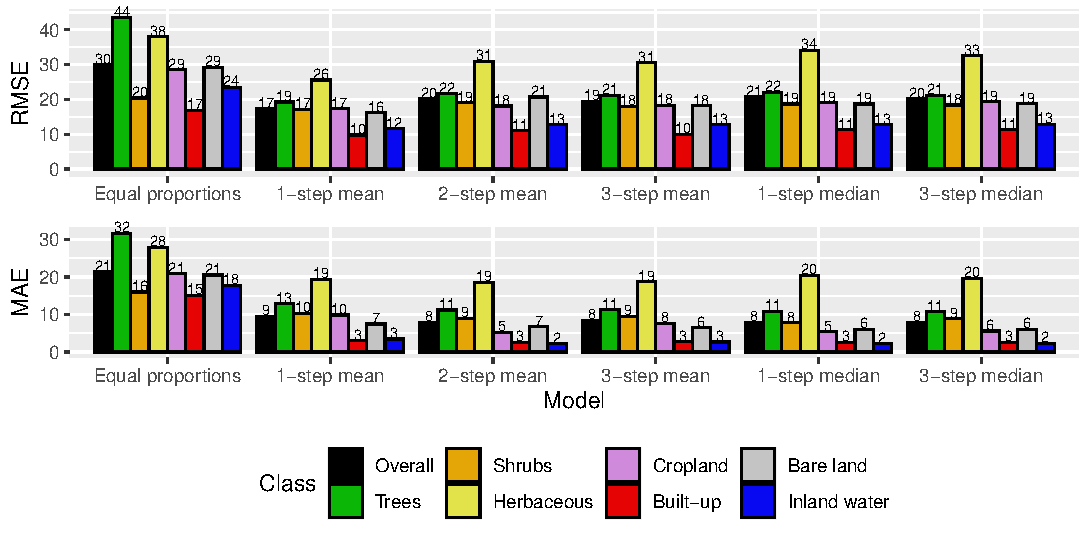
\includegraphics[width=\textwidth]{article-figures/barplots/2020-06-04-rf-comparison-bar}
    \caption{Comparison of \gls{RF} regression models (equal proportion model shown as a reference). 1-step models use no adjustment for zero inflation, 2-step models perform classification on zeroes and regression for non-zeroes, 3-step models perform a classification into pure and non-pure pixels, and then a regression or classification based on that. Mean and median are the tree vote summary statistics.}
    \label{fig-randomforest}
\end{figure}

\subsection{Spatial predictions and accuracy}

To visually demonstrate the predictions of the model with the highest accuracy by \gls{MAE}, we used the three-step median \gls{RF} model to predict land cover fractions at a global scale (100~m resolution, but sampled every 0.2~degrees).
See figure \ref{fig-walltowall} for a visualisation of all of the fraction layers separately, and the supplementary materials for the output GeoTIFF file itself.
The wall-to-wall fraction maps reveal how land cover fraction mapping is capable of expressing gradients and mixed land cover.

In addition, to examine whether there were any patterns in the accuracy of the predictions globally, we produced spatial accuracy maps based on the predictions in locations where we had independent validation data.
This is also presented in raster format in figure \ref{fig-walltowall}.

Biotic gradients can be seen in the global patterns of the land cover fractions.
For instance, gradients are visible between communities dominated by shrubs and ones dominated by herbaceous vegetation, such as in south and east Africa.
Likewise, the gradient of tree cover from 100\% in the African tropics to 0\% in the sub-Sahara region is evident.
The tropical forest edge appears with a hard edge when using median voting and the three-step approach, as forest occurs in discrete patches due to human activity, rather than changing gradually over space.
The tree cover in the transition zone towards savannah is much more mixed and gradual.
Herbaceous cover in sub-Sahara shows an asymmetric gradient: the cover is highest at around 14-15\textdegree{} N and decreases quickly towards the north, becoming zero around 18\textdegree{} N; but decreases slowly towards the south, reaching all the way to 5\textdegree{} N.
Inland water shows up as more discrete, as it naturally forms discrete patches.
Mixed pixels that include water are uncommon.
Built-up area is also relatively rare worldwide.
It rarely forms a 100\% fraction, as urban areas tend to include both built-up area and greenery within the footprint of the 100~m pixel.

The spatial pattern of map accuracy shows that the land cover fractions in areas with pure land cover, such as tropical forests (100\% tree cover) and deserts (100\% bare land), were predicted with the highest accuracy.
Conversely, fractions in areas with mixed land cover were predicted less accurately, as isolating individual fractions from pixel-level information is more challenging.
In addition, land cover fractions in the extreme latitudes were predicted less accurately as well.
In these areas, less training data was available, owing to the lack of high-resolution imagery there.

As we can see from the box widths of the boxplots in figure \ref{fig-walltowall}, the distribution of the predictions was relatively even across the whole range for herbaceous vegetation and trees, but uneven for bare land, inland water and built-up area.
The number of predictions was much more even across the entire range for herbaceous vegetation compared to shrubs.
The model overestimated the fractions of trees and herbaceous cover, as the medians of each box are below the 1:1 line almost throughout the entire range, but it underestimated built-up and crop fractions.
The overall \gls{ME} is below 0.001, which means that overall the model is not biased.

Lastly, we compared the \gls{RF} three-step median model predictions with existing global products that correspond to a particular land cover class in our classification.
The results are given in table \ref{tab-products}.
The \gls{RF} three-step median model performed worse than the \gls{GSW} water occurrence history product, but better than the \gls{GFCC} tree cover and \gls{GHSL} built-up products.
There was a tie when comparing the \gls{RF} three-step median model with the \gls{FROM-GLC} impervious surface product when it comes to \gls{MAE}, but \gls{FROM-GLC} was slightly more accurate according to \gls{RMSE} and less biased according to \gls{ME}.

\begin{sidewaysfigure}
    \centering
    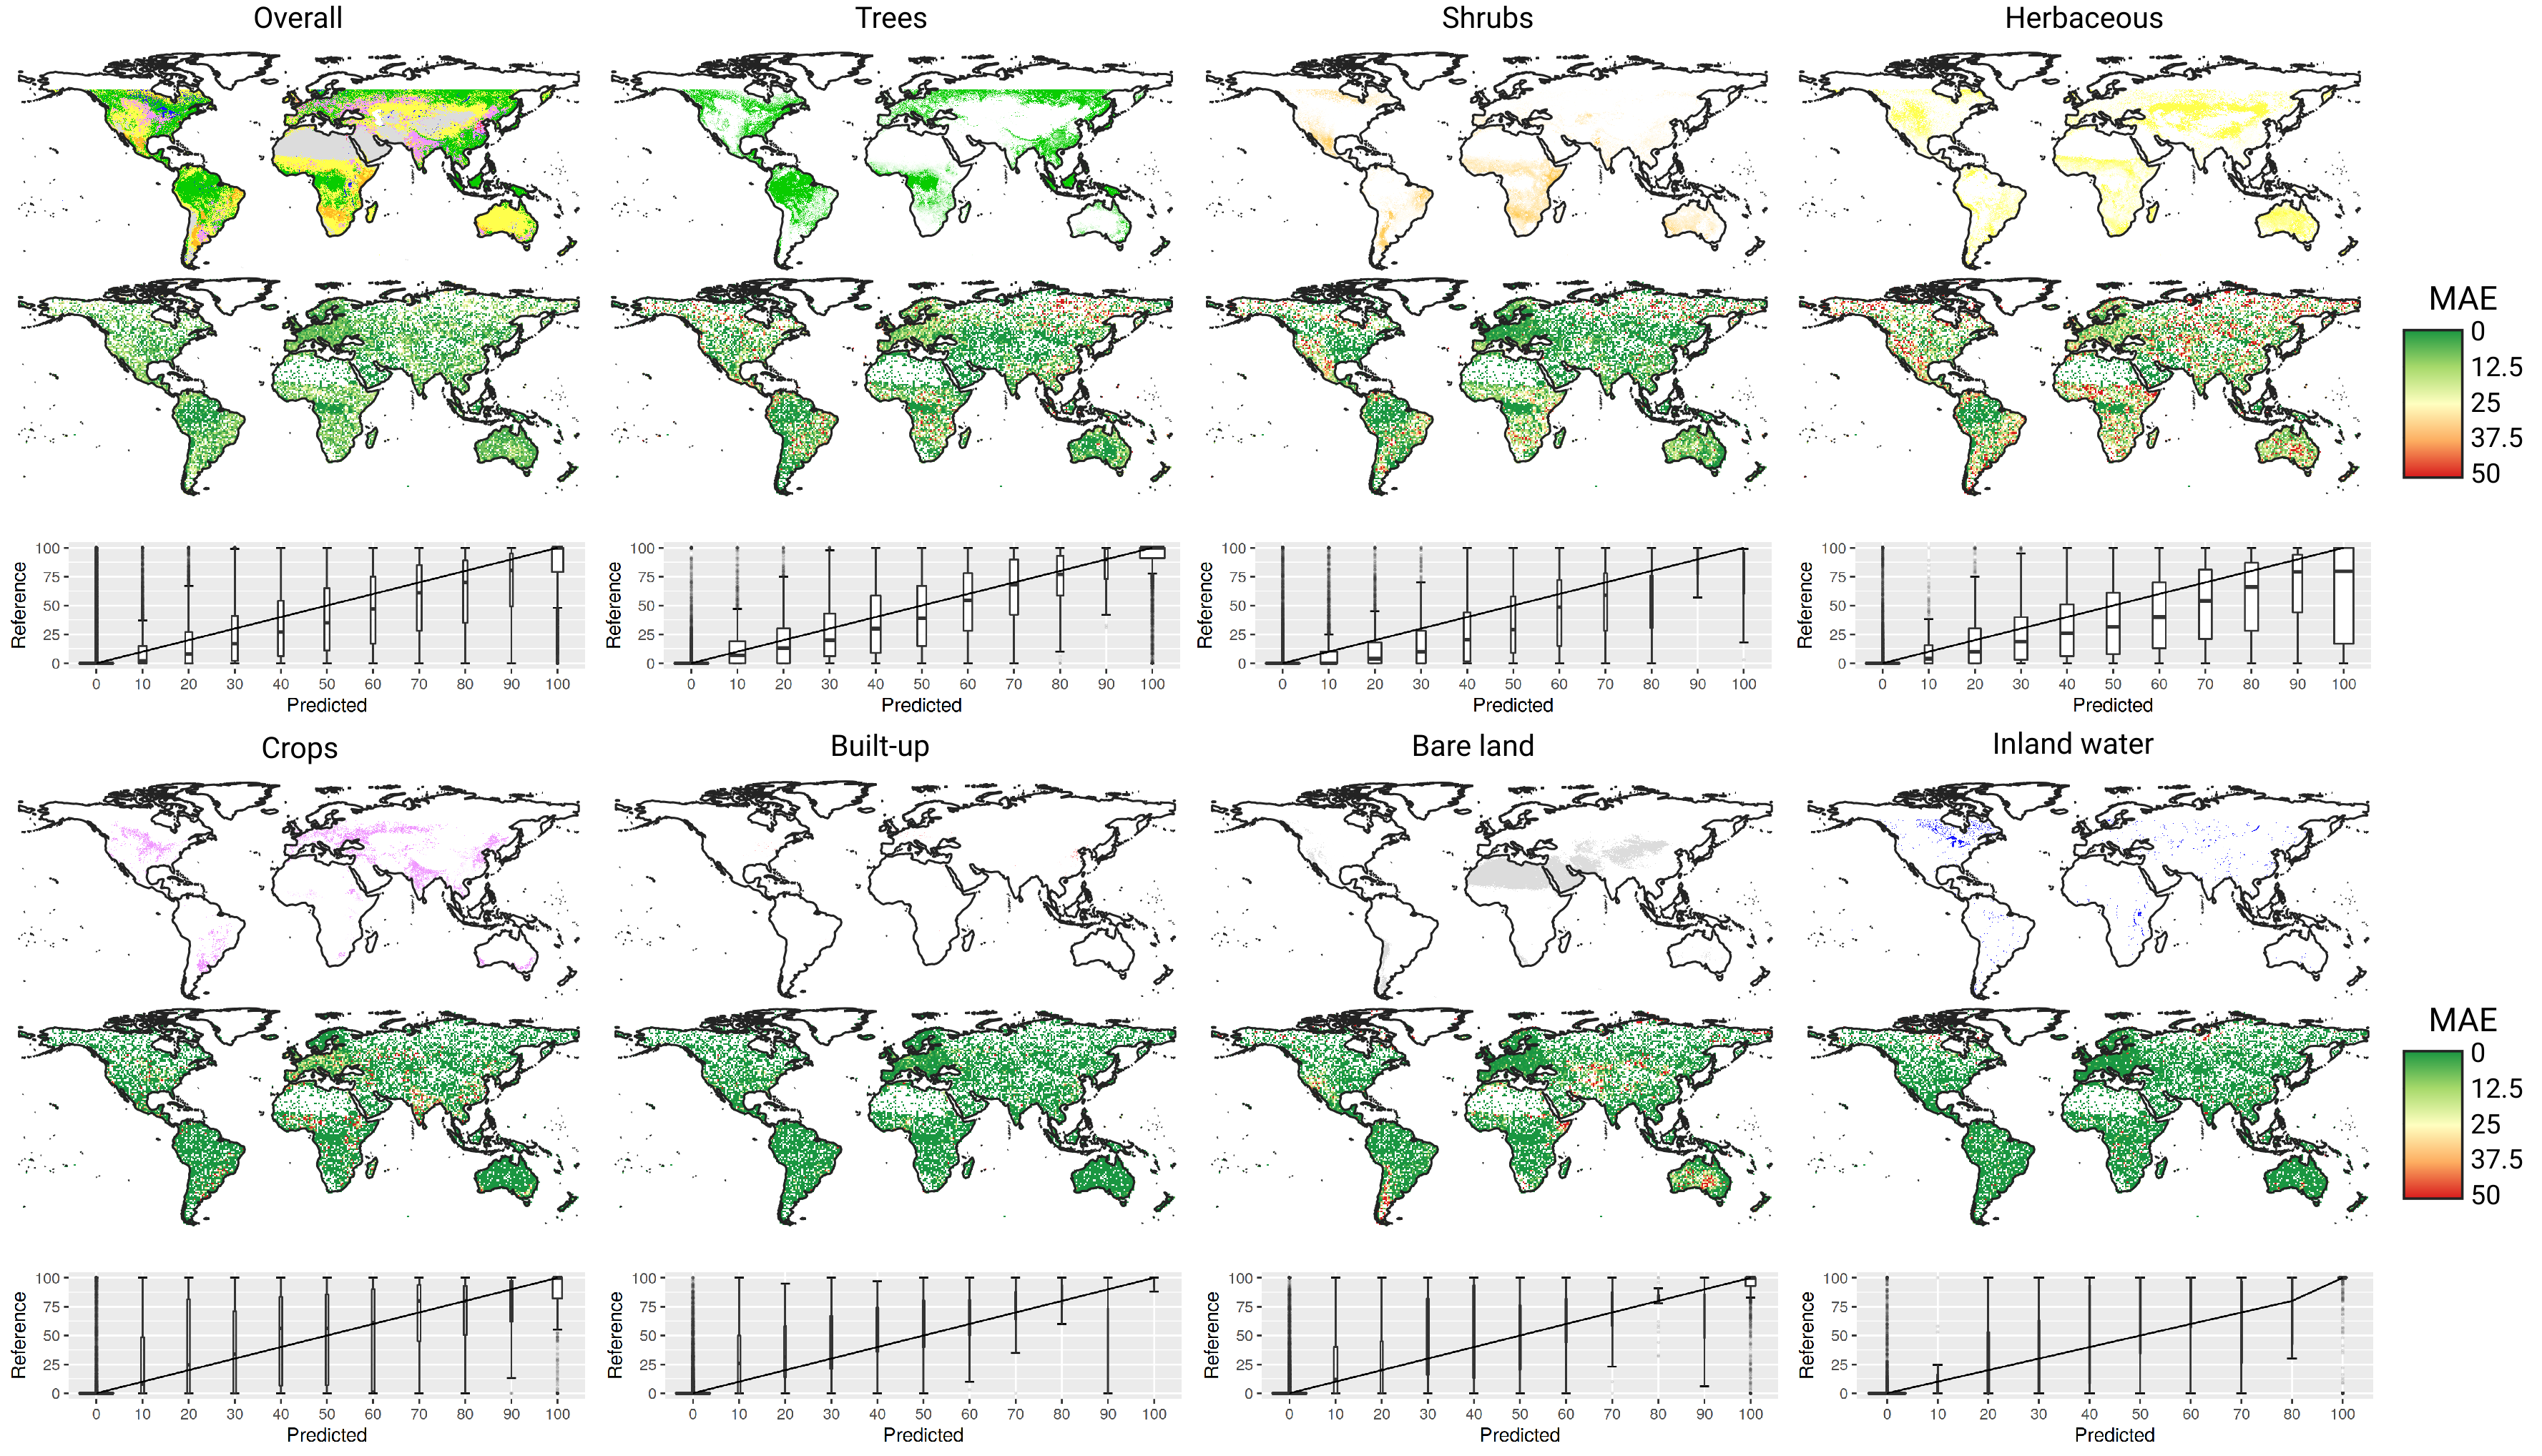
\includegraphics[width=\textwidth]{article-figures/maps/2020-10-12-walltowall.png}
    \caption{Random Forest single model predictions per class. Top row: predicted fractions, each given its own colour (``Overall'' shows a hardened map of dominant land cover using the same colour scheme). Middle row: absolute errors per class, based on predictions at point locations of validation data, displayed aggregated over 1 by 1 degree cells using the mean function. Bottom row: distribution of predicted versus true values, shown as box plots with bins each 10\%, widths representing sample size.}
    \label{fig-walltowall}
\end{sidewaysfigure}

\begin{table}
    \centering
    \adjustbox{max width=\textwidth}{
    \begin{tabular}{lllllllll}
    \toprule
    \textbf{Fraction and source} & \textbf{\glsentryshort{RMSE} (\%)} & \textbf{\glsentryshort{MAE} (\%)} & \textbf{\glsentryshort{ME} (\%)} & \textbf{\glsentryshort{RRMSE}} & \textbf{\glsentryshort{RMAE}} & \textbf{\glsentryshort{RME}} & $\mathbf{R^2_{NSE}}$ & $\mathbf{R^2_{OLS}}$ \\
    \midrule
    %Inland water (RF 1-step) &
    %11.65 & 3.48 & -0.81 &
    %2.07 & 0.62 & -0.14 &
    %0.72 & 0.73 \\
    Inland water (RF 3-step median) &
    12.90 & 2.25 & -1.17 &
    2.29 & 0.40 & -0.21 &
    0.65 & 0.67 \\
    \glsentryshort{GSW}, year 2015 \citep{pekel_high-resolution_2016} &
    \textbf{10.22} & \textbf{1.94} & \textbf{-0.63} &
    \textbf{1.81} & \textbf{0.34} & \textbf{-0.11} &
    \textbf{0.78} & \textbf{0.78} \\
    \midrule
    %Trees (RF 1-step) &
    %\textbf{19.29} & 12.90 & \textbf{-0.56} &
    %\textbf{0.61} & 0.41 & \textbf{-0.02} &
    %\textbf{0.77} & \textbf{0.77} \\
    Trees (RF 3-step median) &
    \textbf{21.18} & \textbf{10.68} & \textbf{1.81} &
    \textbf{0.67} & \textbf{0.34} & \textbf{0.06} &
    \textbf{0.72} & \textbf{0.74} \\
    \glsentryshort{GFCC}, epoch 2015 \citep{townshend_global_2017} &
    28.80 & 18.33 & -12.57 &
    0.91 & 0.58 & -0.40 &
    0.48 & 0.61 \\
    \midrule
    %Built-up (RF 1-step) &
    %\textbf{9.80} & 3.01 & -1.11 &
    %\textbf{3.33} & 1.02 & -0.38 &
    %\textbf{0.38} & 0.51 \\
    Built-up (RF 3-step median) &
    11.28 & \textbf{2.57} & -2.33 &
    3.83 & \textbf{0.87} & -0.79 &
    0.19 & 0.22 \\
    \glsentryshort{GHSL} built-up, 2014 \citep{corbane_ghs-built_2018} &
    18.67 & 5.43 & 4.80 &
    6.34 & 1.84 & 1.63 &
    -1.23 & 0.52 \\
    \glsentryshort{FROM-GLC} impervious surface, 2015 \citep{gong_annual_2020} &
    \textbf{11.18} & \textbf{2.57} & \textbf{0.93} &
    \textbf{3.79} & \textbf{0.87} & \textbf{0.32} &
    \textbf{0.20} & \textbf{0.65} \\
    \bottomrule
    \end{tabular}
    }
    \caption{Accuracy comparison between our results and existing global land cover fraction maps. Highest accuracy and lowest bias results are highlighted.}
    \label{tab-products}
\end{table}

\subsection{Feature importance}

We performed \Gls{RF} permutation importance on the three-step median model to test which features were important for \gls{RF} predictions.
The results are shown in figure \ref{fig-varimp}.

\begin{figure}
    \centering
    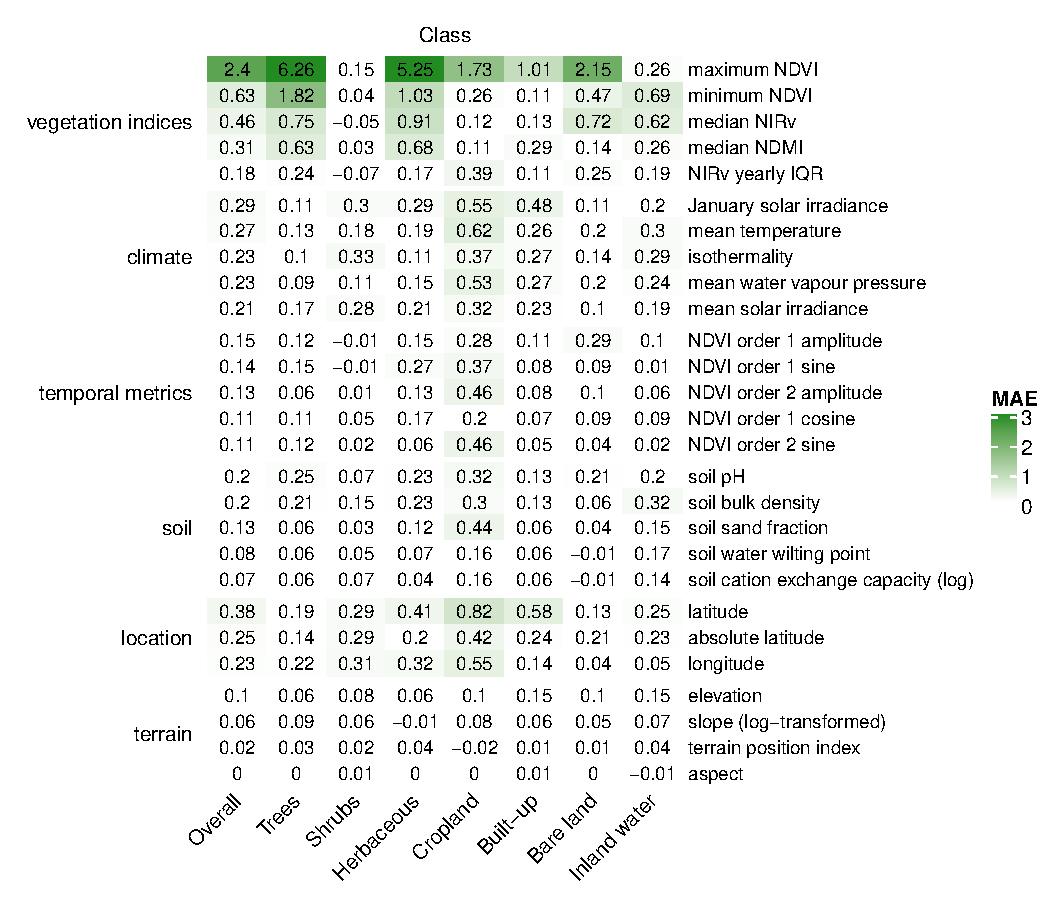
\includegraphics[width=14cm]{article-figures/heatmaps/2020-11-06-varimp-heatmap-top5}
    \caption{Random Forest single-step approach variable importance, top 5 features per category. Categories are ordered by cumulative importance. The values represent increase in MAE for the given class when the given feature is permuted.}
    \label{fig-varimp}
\end{figure}

The overall most important variables were the maximum and minimum \gls{NDVI} over the whole time series of PROBA-V imagery.
They were followed by the median \gls{NIRv} and \gls{NDMI} over the whole time series.
The importance of remote sensing information can also be seen from the accuracy statistics of a single-step \gls{RF} regression model, when only vegetation index and temporal features were input into the model (see table \ref{tab-accuracy}, ``only RS features'').
After excluding all the static features, \gls{RMSE} and \gls{MAE} increased only by around 1 percentage point.

The remote sensing data was of lower importance (and sometimes even confounding) only for the shrub class.
This class is complicated to distinguish from other natural vegetation, and thus when trying to predict shrub cover fractions, the model benefited from a wide variety of additional features, including location and climate information.

To distinguish crops in particular, soil information, such as pH, bulk density and sand fraction, was useful for the model.
Crops are usually grown in fertile soils that can sustain them, and due to the fact that cropland is further managed, the soil is also altered to be more fertile, which affects these soil properties.
In addition, harmonic metrics derived from time series benefited crop cover fraction estimation the most of all the classes.
The second order amplitude and sine of the harmonic model of the time series allows the model to detect areas with a double harvest throughout the year, which is indicative of crops.

Climate data, especially the mean temperature and the closely (exponentially) related mean of water vapour pressure, was also most useful for predicting crop cover fractions.
It was also beneficial for estimating built-up fractions.
Location features were the most important for predicting the cover fractions of these two classes as well.
These classes tend to be spatially clustered, when looking at a large scale.
While the models for predicting the cover fraction of classes made the best use of the location features, all of the classes could benefit from them to some extent, thus it is beneficial to include these intrinsic parameters in the model.
Both absolute and regular latitude were used by the model to improve prediction accuracy, and latitude was more beneficial than longitude for increasing the prediction accuracy.

Terrain information was the least useful feature category.
It was most useful for inland water fraction prediction, since it typically has little to no slope, and rarely occurs at high altitudes.
The aspect was the one feature that does not appear to have contributed to model accuracy.

\section{Discussion}

\subsection{Land cover fraction mapping methods}

In this study, we have tested a number of methods for characterising land cover by means of predicting thematically comprehensive land cover fractions at the global scale.
We found that of the methods that we tested, without additional measures to take the data imbalance into account, \gls{RF} regression and Cubist regression produce output of the highest accuracy by \gls{RMSE} and \gls{MAE}, respectively.
Our findings agree with those of \citet{li_monitoring_2018}, who compared Cubist and \gls{RF} regression for water fraction classification and found that Cubist performs slightly better than \gls{RF} regression for this particular class.
Their Cubist regression result achieved 7.52\% \gls{MAE} and 10.39\% \gls{RMSE}.
Our respective results using Cubist regression were 2.57\% \gls{MAE} and 11.51\% \gls{RMSE}.
While Cubist works best for the inland water class, when considering all of the classes, \gls{RF} regression nevertheless results in higher accuracy (see table \ref{tab-accuracy}).
The difference in the reported numbers may be due to the differences in scale (regional vs global) and training data balance.
As we focused on predicting multiple classes, our training dataset intrinsically had higher zero inflation.

At a local scale, \citet{walton2008subpixelrf} assessed the accuracy of machine learning algorithms for urban land cover fraction mapping and indicated 14.5\% \gls{MAE} and 20.0\% \gls{RMSE} for Cubist, which he also noted as performing better than \gls{RF} regression and \glspl{SVM}.
Our results were 9.70\% \gls{RMSE} and 2.43\% \gls{MAE} for Cubist over the built-up class, and we also noted that Cubist performed slightly better than the other two algorithms for this class.
Both \citet{okujeni_comparison_2014} and \citet{foody1997fuzzynnet} also performed land cover fraction mapping over an urban area.
The results of \citet{okujeni_comparison_2014} indicated that \gls{SVM} regression performed better than \gls{RF} regression.
This could be due to much finer spatial resolution (3.6–9 m) data used in their study, and the associated difference in class definitions.
\citet{foody1997fuzzynnet} reported an \gls{RMSE} of 16.6\% using \gls{MLP} \glspl{NN}, lower than our results (22.7\%).
The differences in the absolute numbers of \gls{RMSE} and \gls{MAE} between these studies and ours are most likely due to the different scope, namely their focus on fine scale predictions over a local area for the urban class in particular, in contrast to our global focus with comprehensive classes, leading to a different balance of the datasets between the studies.

\subsection{Multi-step approach for dealing with data imbalance}

After determining the baseline methods with the highest, we tested our newly proposed multi-step approach on \gls{RF} regression, comparing the effect with that of median voting instead of mean voting.
One challenge in land cover fraction prediction is the tendency of the models to favour the mean over the extremes, as that minimises \gls{RMSE} that may arise from incorrect predictions.
However, that leads to increased fuzziness of the result, where pixels with high uncertainty are marked as a mix of many classes, and fractions of 0\% are rarely, if ever, predicted.
Our proposed multi-step approach adjusts the balance the other way.
As it is a combination of one or two classification models and one regression model, it predicts significantly more pure pixels compared to a single regression model.

Therefore, the multi-step approach was successful in reducing \gls{MAE} (and improving the related \gls{SCM} metrics), as the particularly common case of 0\% fractions was captured better.
On the other hand, it comes at a cost of higher \gls{RMSE} and lower $R^2$.
This is because in highly uncertain, but pure cases, the model makes a best guess of a pure class, and due to the high uncertainty, the prediction is often incorrect.
This leads to 100\% error in those cases, which is highly penalised by \gls{RMSE}.
Due to this effect, the resulting map is closer to a discrete classification map, with less expressive transition gradients between land cover classes.

A similar effect was seen when using techniques such as median voting for \gls{RF} regression.
Median voting also resulted in more correct 0\% fraction predictions, but likewise increased the chances of predicting 100\% of the wrong class.
Our results showed that median voting has a stronger effect for reducing \gls{MAE} than the multi-step approach.
Therefore it may be a suitable choice in cases where it is computationally infeasible to train three models.
However, when the median voting approach was combined with the three-step approach, the \gls{RMSE} decreased without affecting \gls{MAE}.
Thus, three-step median \gls{RF} achieved the best combination that is optimised towards reducing \gls{MAE}, doing so without increasing \gls{RMSE} as much as the single-step median vote model does.

These findings show that the use of a multi-step approach depends on what is more important for the user.
If an occasional prediction of 100\% of the wrong class is acceptable, then a multi-step model provides an overall more accurate result, especially for zero fractions.
On the other hand, a single-step approach emphasises the strength of land cover fraction mapping by expressing gradual changes over space better, and avoids large errors.
The latter is more likely to be useful for the modelling community that deals with uncertainty with probabilistic frameworks, and the former may be more useful for policymakers and land owners who are more concerned with what land cover is most likely to be present on the ground.
In addition, we expect a multi-step approach to be more suitable for fine resolution mapping, where more pure pixels can be expected, and a single-step approach to be more useful for coarse resolution mapping, where mixed pixels are the norm.

It is also worth noting that the multi-step approach is flexible and can be used with any algorithm that provides both classification and regression modes, or with two separate unrelated classification and regression algorithms.
Therefore there may be some combinations of models that have not been tested yet, but could achieve even higher accuracy.

\subsection{Comparison with global land cover products}

To gain insight into how well our proposed multi-step median vote \gls{RF} model performs, we compared it to existing global land cover fraction products.
These products, that only focus on a single land cover class, had varying accuracy compared to our model (see table \ref{tab-products}).
Some products, like \gls{GSW} water occurrence \citep{pekel_high-resolution_2016}, had a higher accuracy.
Others, like \gls{GFCC} forest cover \citep{townshend_global_2017} and \gls{GHSL} built-up \citep{corbane_automated_2019}, had a lower accuracy.
The accuracy of the impervious surface class fraction from \gls{FROM-GLC} mostly matches that of the built-up cover fraction of our proposed model.

The accuracies of other global products reported in literature likewise varied compared to our results.
However, these comparisons are much more difficult to make, as the validation methods and scope vary significantly between the studies.
For example, our \gls{RF} three-step median model had a higher \gls{RMSE} for the tree class (21.1\%) than the one reported by \citet{sexton_global_2013} for their vegetation continuous fields product (16.8\%).
However, \citet{sexton_global_2013} validated their data using lidar datasets within several local study areas, rather than using global image interpretation data as we did.
The study by \citet{montesano_modis_2009} that used a validation approach closer to ours to validate the MODIS tree cover product, reported  an $R^2$ of 0.57, \gls{RMSE} of 13.4\%, RMSD of 21.3\%, slope from a linear regression of 0.5 and intercept of 18.4.
In comparison, our results for the three-step median \gls{RF} model for the tree cover class had an $R^2_{OLS}$ of 0.74, \gls{RMSE} of 21.1\%, slope of 0.87 and intercept of 5.82.
Thus while our model appears to perform better, \citet{montesano_modis_2009} only evaluated boreal regions rather than the entire globe, and used MODIS 500 m data rather than PROBA-V 100 m data.

\subsection{Feature importance}

Remote sensing features were the most important features for the multi-step median \gls{RF} model, especially the maximum and minimum \gls{NDVI} over the entire time series.
Note that these values are taken from a time series that has undergone temporal outlier removal, as detailed in section \ref{sec-temporal-filter}, and thus roughly correspond to the 5th and 95th percentiles of the data without additional temporal filtering.
Multiple vegetation indices were useful for increasing the model accuracy: both \gls{NDMI} and \gls{NIRv} median over the time series were much more important than any other feature from other groups.
Nevertheless, even though a lot of the other features were of much lower importance, they contributed to prediction accuracy enough so that they could not be easily excluded from the models as redundant (after the removal of collinear features as explained in section \ref{sec-covariate-selection}).
Methods based on decision trees help with effectively using features that may also have an overlap in the information that they provide, although linear models likewise tended to not exclude any features as non-informative.
This is also due to the large variety of land cover classes in the study, since a feature is useful if it helps predict any of the land cover classes better.

The result that including more training features is beneficial, but remote sensing data is the most important, is in line with the conclusions of e.g. \citet{li_monitoring_2018} and \citet{hengl_soilgrids250m_2017}.
Remote sensing data is also unique in that it forms a time series, which enables us to both calculate additional temporal metrics and to monitor land cover change over time.
In addition to remote sensing data, \citet{hengl_soilgrids250m_2017} also noted high importance of climate data, however, it is focused on soils, whereas climate has more effect on long-term processes such as soil formation than on land cover.
Climate data was the second most important in our case, mostly for the crop fraction estimation, which is also closely linked with soils.
Note that the feature importance may be different at different scales, e.g. if predictions are made at a finer spatial resolution, such as 30~m or 10~m.

\subsection{Challenges and future outlook}

Machine learning algorithms pose several challenges that are inherent to how the models are constructed.
The trade-off between minimising \gls{RMSE} and minimising \gls{MAE} comes from the chosen loss function.
Typically, in cases of high uncertainty, the loss function is minimised when the predictions tend towards the mean.
In that case, the models predict in areas with a high cover of a fraction, such as mixed shrublands, a lower fraction of the class than expected, whereas in cases with a low cover, such as for fraction of built-up, higher fractions are predicted than expected.
This is due to a prediction of the mean being less penalising than predicting the extremes incorrectly; e.g. for a case of 50\% shrub cover, predicting 100\% shrubs would be a larger mistake (and thus lead to higher \gls{RMSE}) than predicting 15\% shrubs.
Likewise, predicting 0\% built-up in areas covered by dark bare soils risks a case where it truly would be 100\% built-up, so on average predicting 15\% built-up in this case lowers the possible error.
The three-step approach (or median vote) tilts the balance in the other direction, as e.g. the first step determines that the pixel is pure, and the classification step determines that it is more likely to be bare soil than built-up area.
But there may also be cases when the classifier predicts the wrong class.
If the pixel is not pure, the regression step still tends to predict towards the mean due to the loss function, so the challenge of underestimating large fractions and overestimating small ones remains.
However, with the multi-step approach, it is now possible to influence the decision process of the model to tweak it towards the desired outcome.
In addition, using a median vote in tree-based ensemble models makes the model tend towards the median, which may still be one of the extreme values.
In that case, the model typically overestimates or underestimates values for most of the value range, but on average is still not biased, as the predicted values are more polarised but balance each other out.
The multi-step approach could be improved further by exploring the option of using different machine learning models for each step, and by gathering more features that would increase the accuracy of the models at each of the steps.

There is another inherent challenge in land cover mapping for discerning classes that are related, e.g. herbaceous vegetation and shrubs.
These classes were particularly difficult to map, in part due to their heterogeneity, and in part due to confusion between herbaceous vegetation, cropland and shrubs.
As shown in figure \ref{fig-varimp}, specific types of features can be used to discriminate between these classes better.
Specifically, the identification of herbaceous vegetation is primarily based on vegetation indices, identification of shrubs relies mostly on climate data, whereas cropland identification is more data-intensive and makes use of vegetation indices, temporal metrics, climate, soil and location information.
These three classes are challenging to discriminate between not just for regression algorithms, but also for expert interpreters, which may lead to higher uncertainties also in the training and validation data for these classes.
It is even more challenging to discern between these classes if they mix within the area of a single pixel, which is common in grasslands and shrublands, as well as in smallholder agriculture.
The difference between the definition of trees, shrubs and herbaceous vegetation largely comes down to plant height, therefore dynamic information about vegetation height would allow mapping these classes more accurately.
However, this would require either photogrammetry techniques (that typically rely on much finer spatial resolution and more overlap between the scenes) to reconstruct vegetation height, or the use of non-optical sensors such as \gls{SAR} interferometry.
Another way to differentiate between the vegetation classes could be to make use of hyperspectral data, which allows differentiation between different kinds of vegetation based on e.g. their photosynthesis processes or water content, which affect light absorption.
Emerging new high level hyperspectral products, such as \gls{SIF} or \gls{GPP}, such as ones based on the upcoming FLEX satellite, could allow for a straightforward way to incorporate this extra information into land cover models.
Hyperspectral data could be useful for better differentiation of non-vegetated classes as well, such as bare soil from urban, e.g. by separating the spectral signature of sand from concrete or asphalt.
In addition, land cover time series information could help track land cover change over time, as the land cover at one time step depends on the land cover at the previous step.
This information would allow the regressor to limit the predicted values to a smaller range, and thus reduce the noise in the predictions.

Another challenge is class imbalance.
For example, the built-up class rarely forms a 100\% fraction.
That makes it simple to achieve a high prediction accuracy according to absolute statistics, as a fraction of 0\% is in most cases not far off from the true value.
However, a prediction of 0\% in every pixel makes the fraction map not useful for user needs.
This challenge is further exacerbated by the training dataset containing relatively few points in built-up areas to begin with.
Therefore, having a more balanced training dataset may further increase the accuracy of the models.
However, the issue of value imbalance within the class will always remain for land cover fraction mapping, therefore the multi-step model approach will be relevant, especially if the legend involves even more classes, or if the land cover is more homogeneous at the level of the mapping unit.

In this study, model optimisation and dataset sizes were also a challenge.
Each model may have multiple parameters that can be tuned, and the input to each method can also be modified (e.g. by log-transforming features or replacing missing values).
Since the large dataset size increases the training time for the models, parameters to tune have to be chosen carefully.
As such, it is possible to miss a particular parameter combination that may further improve the results.
On the other hand, our results showed that the differences between the best performing methods are not very high.
The differences in model parametrisations are expected to be even lower.

Another challenging aspect about land cover fraction mapping is the available algorithms that would suit this use case.
In its core, it is a multivariate regression problem, but most regression algorithms are univariate.
Our results showed that the binary relevance method works well to facilitate the use of univariate regression methods for this task, as the highest accuracy was achieved by algorithms that used the binary relevance method.
This further expands the field of possible algorithms that could be used.
In addition, both the binary relevance method and the multi-step method can accept different algorithms for its submodels, i.e. for different classes in the case of binary relevance and for different steps in the case of the multi-step approach.
There may be a combination of models that would work even better than the models we tested.
We could not cover the entire range of methods in the scope of this study, therefore there is still room for improvement.
For example, classical spectral unmixing methods, such as spectral mixture analysis, has been often used in the past (e.g. in \citet{adams_classification_1995}).
However, due to the limitations of the spectral mixture analysis methods \citep{somers_endmember_2011}, we could not use it with the features we selected (as listed in the supplementary material, table S1), as they do not form a linear mixture representing the land cover fractions.
Modern machine learning methods are advantageous for their ability to model complex nonlinear relationships between variables and thus make use of all of the features as shown in figure \ref{fig-varimp}.

The scale of the study poses performance challenges, as features that the models use need to be available at a global scale.
Our results showed that all of the feature groups used in the study were useful, therefore leaving a feature out means sacrificing some predictive power.
The gain would be less time needed for processing, as that feature would no longer need to be downloaded, preprocessed and processed.
In addition, model training performance (time for training and memory usage) may be an important consideration for global land cover mapping, as it may limit the scope of what models may be used for this task.
For example, ensemble learning techniques like the super learner are very resource-intensive and may take weeks to train.
Therefore it is important to take into account not just the model accuracy, but also whether the improvement of the accuracy is worth the increase in processing time or computing resource usage.

Several more challenges are yet to be tackled in this field, but doing so is becoming more and more feasible over time.
%Studies on methods such as ours contribute to increasing the accuracy of land cover products and making them more suitable for target user audiences, without the need of gathering and processing additional data.
%The three-step method proposed and described in this study has already been adopted in production of the \gls{CGLS-LC100} product.
%While this study presents the original idea of, and independent research into, the multi-step method, \citet{buchhorn_copernicus_2020} describes how the method was applied in the production process of the \gls{CGLS-LC100} product.
%
Finer spatial resolution mapping, such as 10 m mapping using Sentinel-2 data, is a future research direction, where the pixel footprint will more likely cover homogeneous land.
Therefore, due to an increase in 0\%/100\% fractions, such future developments would be more likely to benefit from a multi-step approach or optimisation for \gls{MAE}.
The multi-step approach is fully portable to finer scales, but more research is needed to determine the effect of the different scales on the purity of the pixels, and how much benefit does a combination of classification and regression bring compared to doing only classification or only regression.
Finer spatial resolution sensors can also be used for mapping fractions at coarser resolutions in a more precise way, by performing aggregation of the finer resolution pixels to estimate the land cover fraction at a coarser resolution.
This is likely to become the norm if even finer resolution data (e.g. 1~m) becomes available globally.

Another benefit of using different optical sensors is higher spectral resolution.
As PROBA-V only measures four spectral bands, the amount of information that can be retrieved from them is limited.
Sensors such as Sentinel-2 \gls{MSI} have a much wider range of spectral bands that could be used both directly as features, as well as enable computing a more diverse range of \glspl{VI}, such as ones based on the slope of the red edge.
This could potentially improve the distinction between different land cover classes.

With more availability of such additional remote sensing data, it becomes increasingly more feasible to perform land cover monitoring and change mapping.
Mapping land cover fractions is a great opportunity to track gradual changes, such as regrowth, better.
The challenge here is that the higher uncertainty about fraction estimates may cause the time series of land cover fractions to fluctuate, making it difficult to determine robust trends.

\section{Conclusions}

In this study, we compared multiple groups of algorithms for land cover fraction mapping.
The best performing models were based on \gls{CART} tree ensembles, with \gls{RF} regression performing the best overall.
A single-step \gls{RF} regression model using majority voting resulted in the best results for RMSE (17.3\%) and $R^2_{NSE}$ (0.66).
In addition, we investigated ways to tackle the issue of accurately predicting the extreme fraction values of 0\% and 100\% by proposing a hierarchical multi-step approach combining classification and regression models.
We compared and combined this approach with \gls{RF} median voting.
The combined \gls{RF} median three-step approach obtained the best results for \gls{MAE} (7.9\%) and \gls{SCM} \gls{OA} (72±2\%).
Based on this model, we created a demonstration map showing the global distribution of land cover in separate land cover fraction layers.
Remote sensing features were the most important for model accuracy, although all other types of features (climate, soil, terrain) also contributed significantly.

These findings directly contribute to the operationalisation of global land cover fraction mapping by analysing and advancing currently available methods for thematically exhaustive global land cover fraction mapping.
Information on land cover fractions offers better precision than discrete land cover maps, and allows the users to manually define thresholds to generate discrete classifications of their own choosing, based on their classes on interest.
Furthermore, given the recent advances in optical sensor spatial resolution and the resulting increase in pixel purity, the multi-step model approach may become more important in the future.
Lastly, due to the advances in spatial and spectral resolution, longer imagery time series of existing sensors, and the availability of non-optical sensor data, this work paves the way towards operational land cover fraction change mapping, which would allow monitoring gradual land cover change.

% Converted from role-centric to person-centric as per Elsevier guidelines: https://www.elsevier.com/authors/journal-authors/policies-and-ethics/credit-author-statement
%\minisection{Author Contributions}
%\textbf{Dainius Masiliūnas}: Methodology, Formal Analysis, Software, Writing – Original Draft, Data Curation. \textbf{Nandin-Erdene Tsendbazar}: Investigation, Data Curation, Supervision, Conceptualisation, Writing – review \& editing. \textbf{Martin Herold}: Conceptualisation, Project Administration, Supervision, Methodology. \textbf{Myroslava Lesiv}: Investigation, Data Curation. \textbf{Marcel Buchhorn}: Writing – review \& editing. \textbf{Jan Verbesselt}: Conceptualisation, Methodology, Supervision, Writing – review \& editing.

\minisection{Acknowledgements} We would like to thank VITO and Terrascope for providing us with computational facilities to access and process {PROBA-V} data, and IIASA for providing the model training dataset. In addition, we thank Bruno Smets for ideas and support from the \gls{CGLS-LC100} project, Benjamin Kellenberger for help on tuning \gls{NN} parametrisation, as well as Linlin Li and Tomislav Hengl for suggestions on additional machine learning methods to test. We also thank the three anonymous reviewers for their valuable and detailed comments.

% NOTE: Appendix is in supplement.tex

%\section*{Abbreviations}

%\printnoidxglossary[type=acronym]

\bibliography{article-bib}

%\listoffigures

\end{document}
